\chapter{Previsão de cintilação ionosférica com 1h de antecedência}\label{ch:revisonrezende}

A primeira parte deste capítulo discute o trabalho \cite{REZENDE:2009}. A segunda expande e generaliza os problemas discutidos por este.

\section{Revisão do trabalho \cite{REZENDE:2009}}

O trabalho \cite{REZENDE:2009} foi pioneiro na utilização de modelos direcionados por dados para o tratamento do problema de previsão cintilação ionosférica, entretanto este trabalho não apresenta uma abordagem completamente reprodutível, visto ausência dos códigos e da base de dados. O objetivo desta revisão é entender as dificuldades deste trabalho, assim como sua incompletude em relação a proposta a ser estabelecida nessa monografia.

\subsection{Principais Pontos}

A previsão de cintilação de curto prazo (uma hora) foi realizada utilizando {\bf amostras com intervalos de 5 minutos}, entretanto alguns dos atributos apresentam resolução inferior, sendo portanto interpolados, ou copiados de sua vizinhança, enquanto outros apresentam resolução mais altas, e neste caso precisaram ser agrupados segundo algum critério, por exemplo, por uma operação de máximo.

Os atributos foram:

\begin{itemize}
\item {\bf Hm\_Eq} representa a hora no equador (em São Luis), em intervalos de 5 minutos;
\item {\bf Vel\_Der} é a velocidade máxima de deriva vertical do plasma medida no equador entre as 17-19 LT (20-22 UT), com resolução de um valor por dia;
\item {\bf Kp} é a média do índice Kp definido pela expressão:
\begin{equation}
\sum_{i=1}^{n}\sum_{j=1}^{i}\frac{Kp_{j}}{ni}\mbox{,}~
\end{equation}
onde $Kp_1$ corresponde ao Kp medido entre 14-17 LT, $Kp_2$ entre 11-14 LT, até o valor medido entre 5-8 LT, o valor de $n$ é 4. Este valor apresenta resolução diária;
\item {\bf F10.7} é o fluxo solar, com resolução de uma medida por dia;
\item {\bf S4\_Eq} é o maior valor do índice S4 medido no equador, em um período de 5 minutos;
\item {\bf S4\_PA\_tempo\_real} é o maior valor do índice S4 medido no pico da anomalia (São José dos Campos), em um período de 5 minutos;
\item {\bf S4\_PA} é o S4 estimado com uma hora de antecedência para o pico da anomalia, com resolução de 5 minutos.
\end{itemize}

As primeiras 5 variáveis correspondem aos atributos preditores, enquanto a variável {\bf S4\_PA} corresponde ao atributo reposta. Os atributos acima passam por algum pré-processamento antes e depois da seleção das amostras:

\begin{itemize}
\item $S_4$: antes da seleção, somente são utilizados os valores medidos para satélites com ângulo superior a 30 graus;
\item $S_4$: depois da seleção, a grande variabilidade dos dados de $S_4$ levam a adoção de um filtro passa baixa para as variáveis {\bf S4\_Eq}, {\bf S4\_PA\_tempo\_real} e {\bf S4\_PA} (variáveis definidas em termos do índice $S_4$), realizado por meio de uma suavização com média móvel com janela 15 pontos;
\item Kp: depois da seleção, somente são mantidos amostras com valores de Kp inferiores a 3, pois valores maiores que este caracterizam forte pertubação magnética. Estas por sua vez estão associadas a eventos extremos como tempestades magnéticas, nesta configuração a predição se torna inviável.
\end{itemize}

Os dados depois da seleção, devem compreender o período  entre as 18-23LT (21-01UT) de forma a predizer os valores no intervalo 19-24LT (22-02UT).

Ao final, a base de dados deste trabalho apresentava um total de 80 dias de dados com 4680 amostras, coletadas entre 2000 e 2002. Este trabalho também realizou testes com predições com 1 dia de antecedência, entretanto estes não apresentaram um resultado tão significativo e, portanto, não serão discutidos.

Restam definir dois elementos para que o problema fique completamente definido, as métricas, e os modelos. Uma vez que as métricas ficam restringidas segundo os modelos, ir-se-á estabelecer estes primeiros:

\begin{itemize}
\item agrupamento por expectation-maximization implementado no ambiente Weka;
\item regras de associação utilizando o algoritmo apriori, onde neste caso os atributos foram discretizados;
\item regressão, utilizando árvores CART com a técnica de conjunto bagging, implementadas pelo autor. Algoritmo análogo à Floresta Randômica.
\end{itemize}

As métricas adotadas foram o erro quadrático médio, e o índice de correlação de Pearson para o problema de regressão, e inspeção para as demais. A aplicação de agrupamento permitiu concluir que se tratava de um problema altamente não linear, as regras de associação geram conclusões que já eram bem conhecidas da literatura do problema em aeronomia. Finalmente, os resultados mais interessantes foram estabelecidos pelo problema de regressão, com erro quadrático médio de 0.05 com correlação de Pearson de 0.985.

O trabalho foi uma abordagem inédita para o problema da predição da cintilação ionosférica.

\subsection{Análise}

A análise consistiu em levantar e sintetizar alguns pontos que levam a uma definição parcialmente incompleta do problema, ou talvez errônea do mesmo:

\begin{enumerate}
\item uma vez que o código e a base de dados não é disponibilizada de maneira pública e nem devidamente documentada, a reprodução somente é possível em partes. Visto que serão utilizados algoritmos que muito se assemelham, esperam-se resultados de mesma ordem, entretanto devido as diferenças resultados que divirjam podem ocorrer;
\item do ponto de vista de implementação não foi definido uma representação para a variável {\bf Hm\_Eq}. Esta pode ser então representada em segundos, minutos, entre outras opções, entretanto note que isto não deveria levar a diferenças significativas no resultado final;
\item a variável Kp é medida por padrão nos intervalos 00-03 UT, 03-06 UT, 06-09 UT, 09-12 UT, 12-15 UT, 15-18 UT, 18-21 UT e 21-24 UT, e não nos intervalos utilizados pelo autor, sendo portanto necessário definir como é feito este mapeamento, o que não está presente no texto;
\item a definição de como a média móvel é aplicada na quantidade S4 está um tanto incompleta, isto é, dado o i-ésimo elemento de um vetor, com um tamanho de janela de 15 pontos, ela poderia ser aplicada levando-se em consideração: os 14 pontos anteriores, $\{i-14, i-13, ..., i-1, i\}$; ou os 7 pontos anteriores e 7 posteriores, $\{i-7,...,i-1,i,i+1,...,i+7\}$, denominada de forma central; entre outras combinações;
\item levando em consideração que a forma centrada tenha sido adotada, a janela de 15 pontos exigirá que 7 pontos do futuro sejam conhecidos, neste caso, dado um instante $t$ seriam necessários 35 minutos de dados a frete deste para o cálculo da média e,  portanto, na verdade, o resultado não seria previsto com uma hora de antecedência, mas sim 25 minutos;
\item a métrica, erro quadrático médio, pode não contemplar o problema. Para entender tal proposição, considere a adaptação deste problema para uma classificação, ficará evidente que eventos com altos valores de cintilação são mais raros e, portanto, ter-se-á um problema de classificação não balanceado. Retornando, a regressão, pode-se ocorrer do modelo predizer muito bem valores baixos, que então irão mascarar os efeitos de erros em valores mais altos, visto que irão predominar no processo de cálculo de média.
\end{enumerate}

\section{Reprodução}\label{se:rep}

O trabalho \cite{REZENDE:2009} foi parcialmente, reproduzido no contexto desta proposta, pois somente uma linha de pesquisa do trabalho original foi explorada: o problema de regressão, e cuidados adicionais foram necessários, devido a utilização de mais anos, entretanto o total de amostras com todos os atributos não nulos ficou reduzido devido a presença de grandes lacunas nos dados. As Figuras \ref{fig:distribution} e \ref{fig:nulltotal} mostram respectivamente a distribuição dos dados ao longo do conjunto de amostras, onde espaços em brancos representam valores ausentes e a razão e o total de dados não nulos.

\begin{figure}[H]
\centering
\makebox[\textwidth][c]{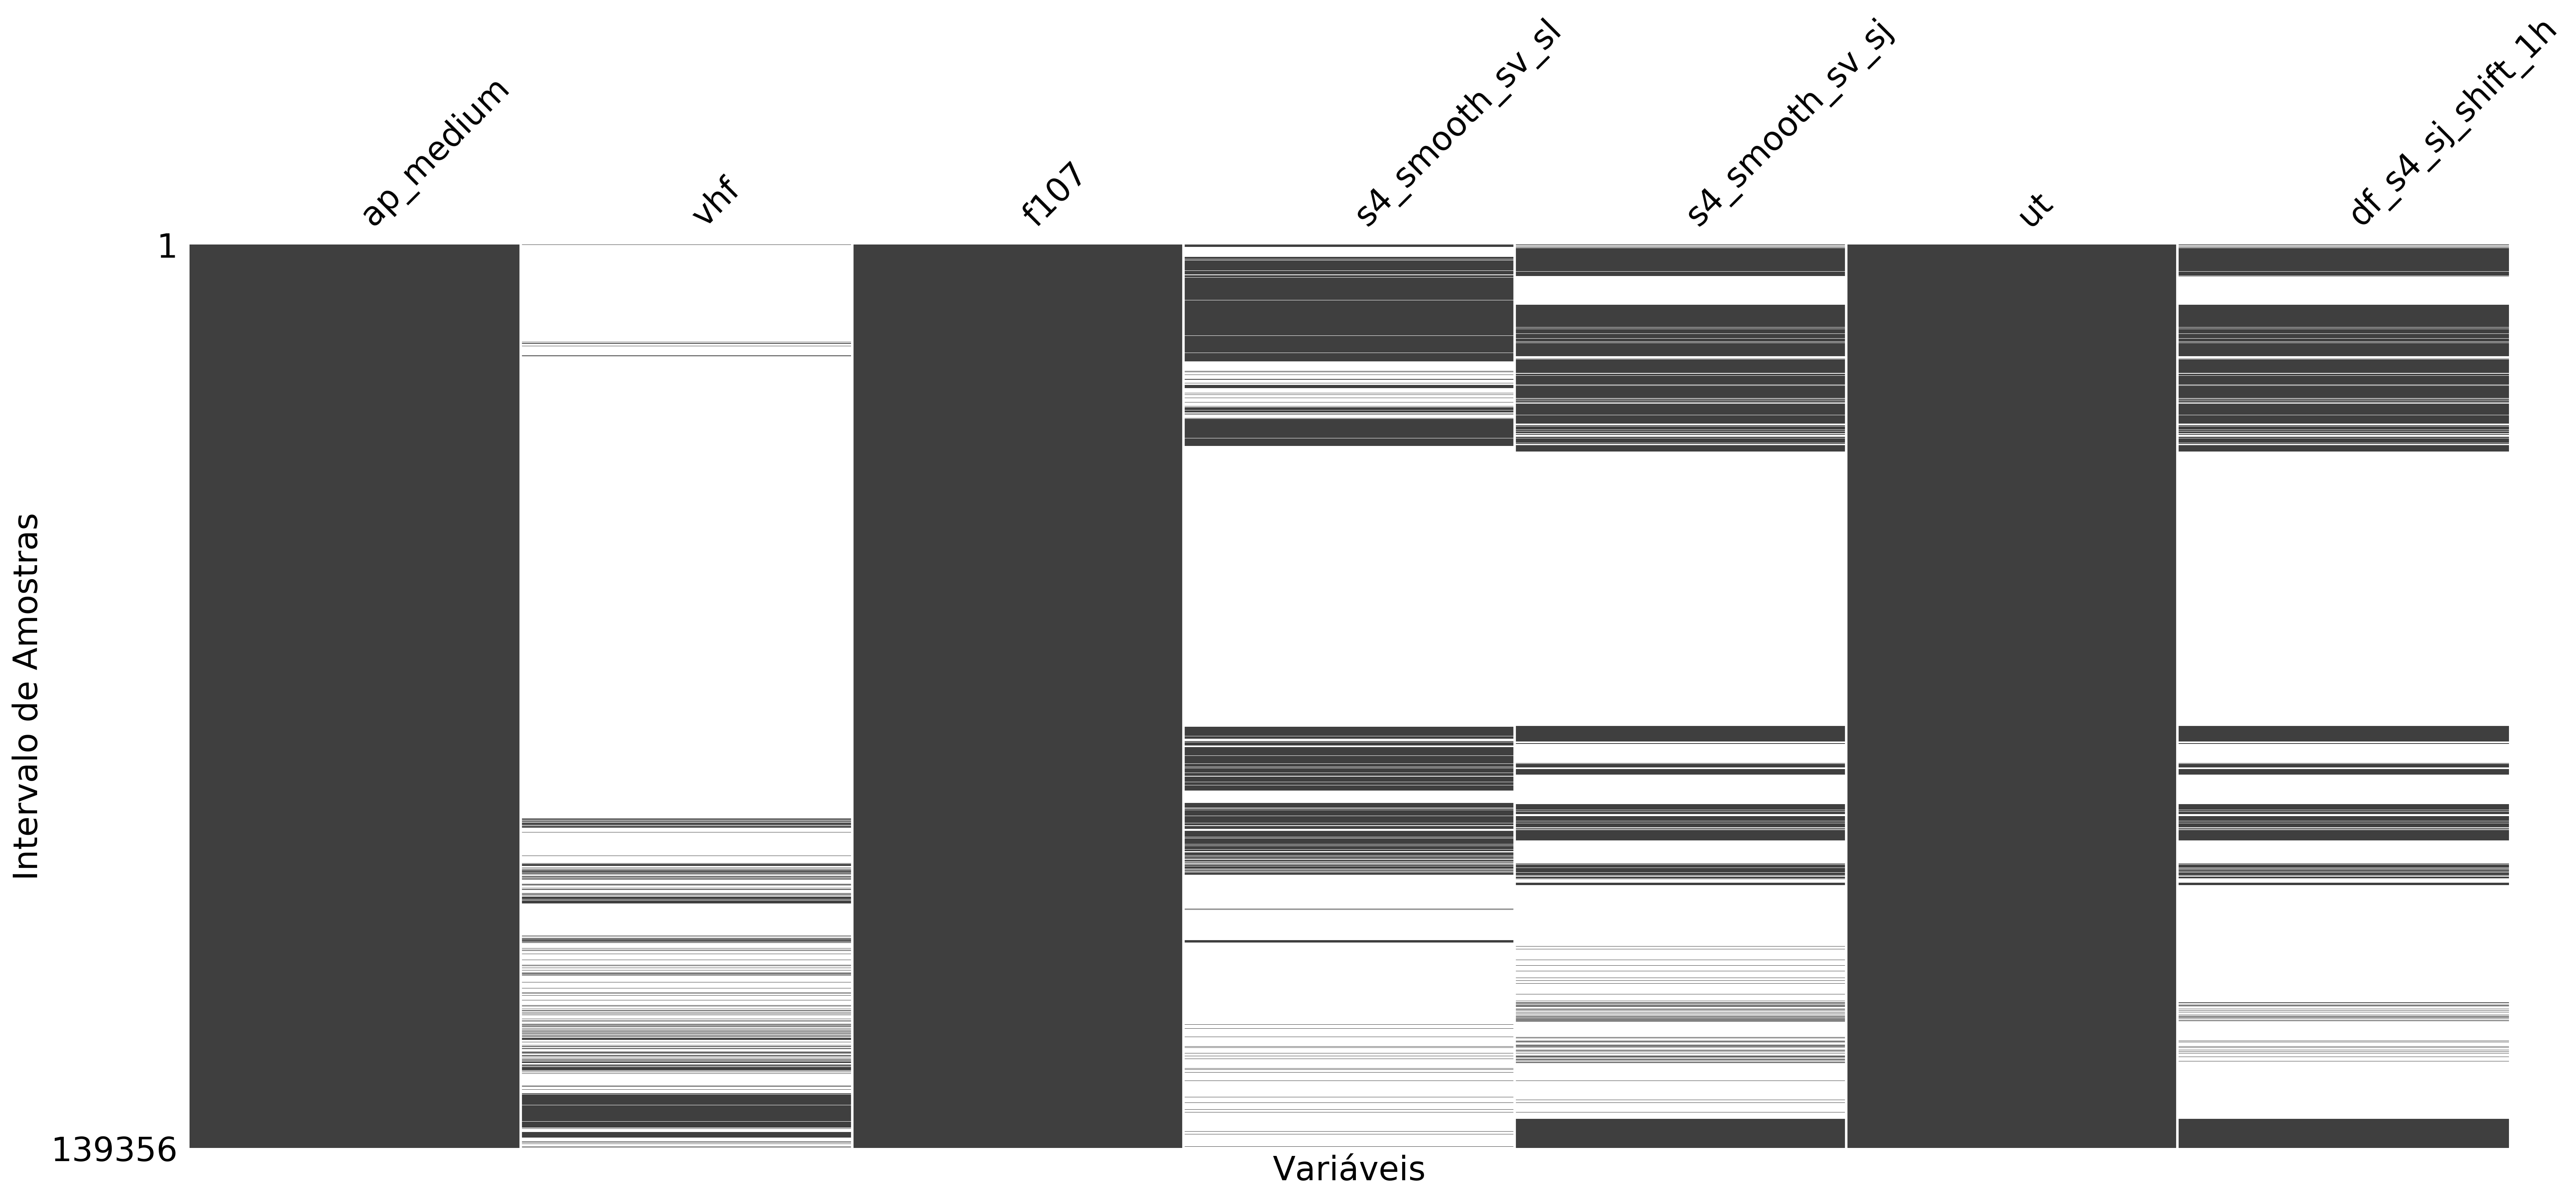
\includegraphics[width=1.2\linewidth]{./Figuras/results-original/distribution.eps}}
\caption{Distribuição dos dados ao longo do conjunto de amostras. Espaços em brancos representam valores ausentes. Fonte: próprio autor.}
\label{fig:distribution}
\end{figure}

\begin{figure}[H]
\centering
\makebox[\textwidth][c]{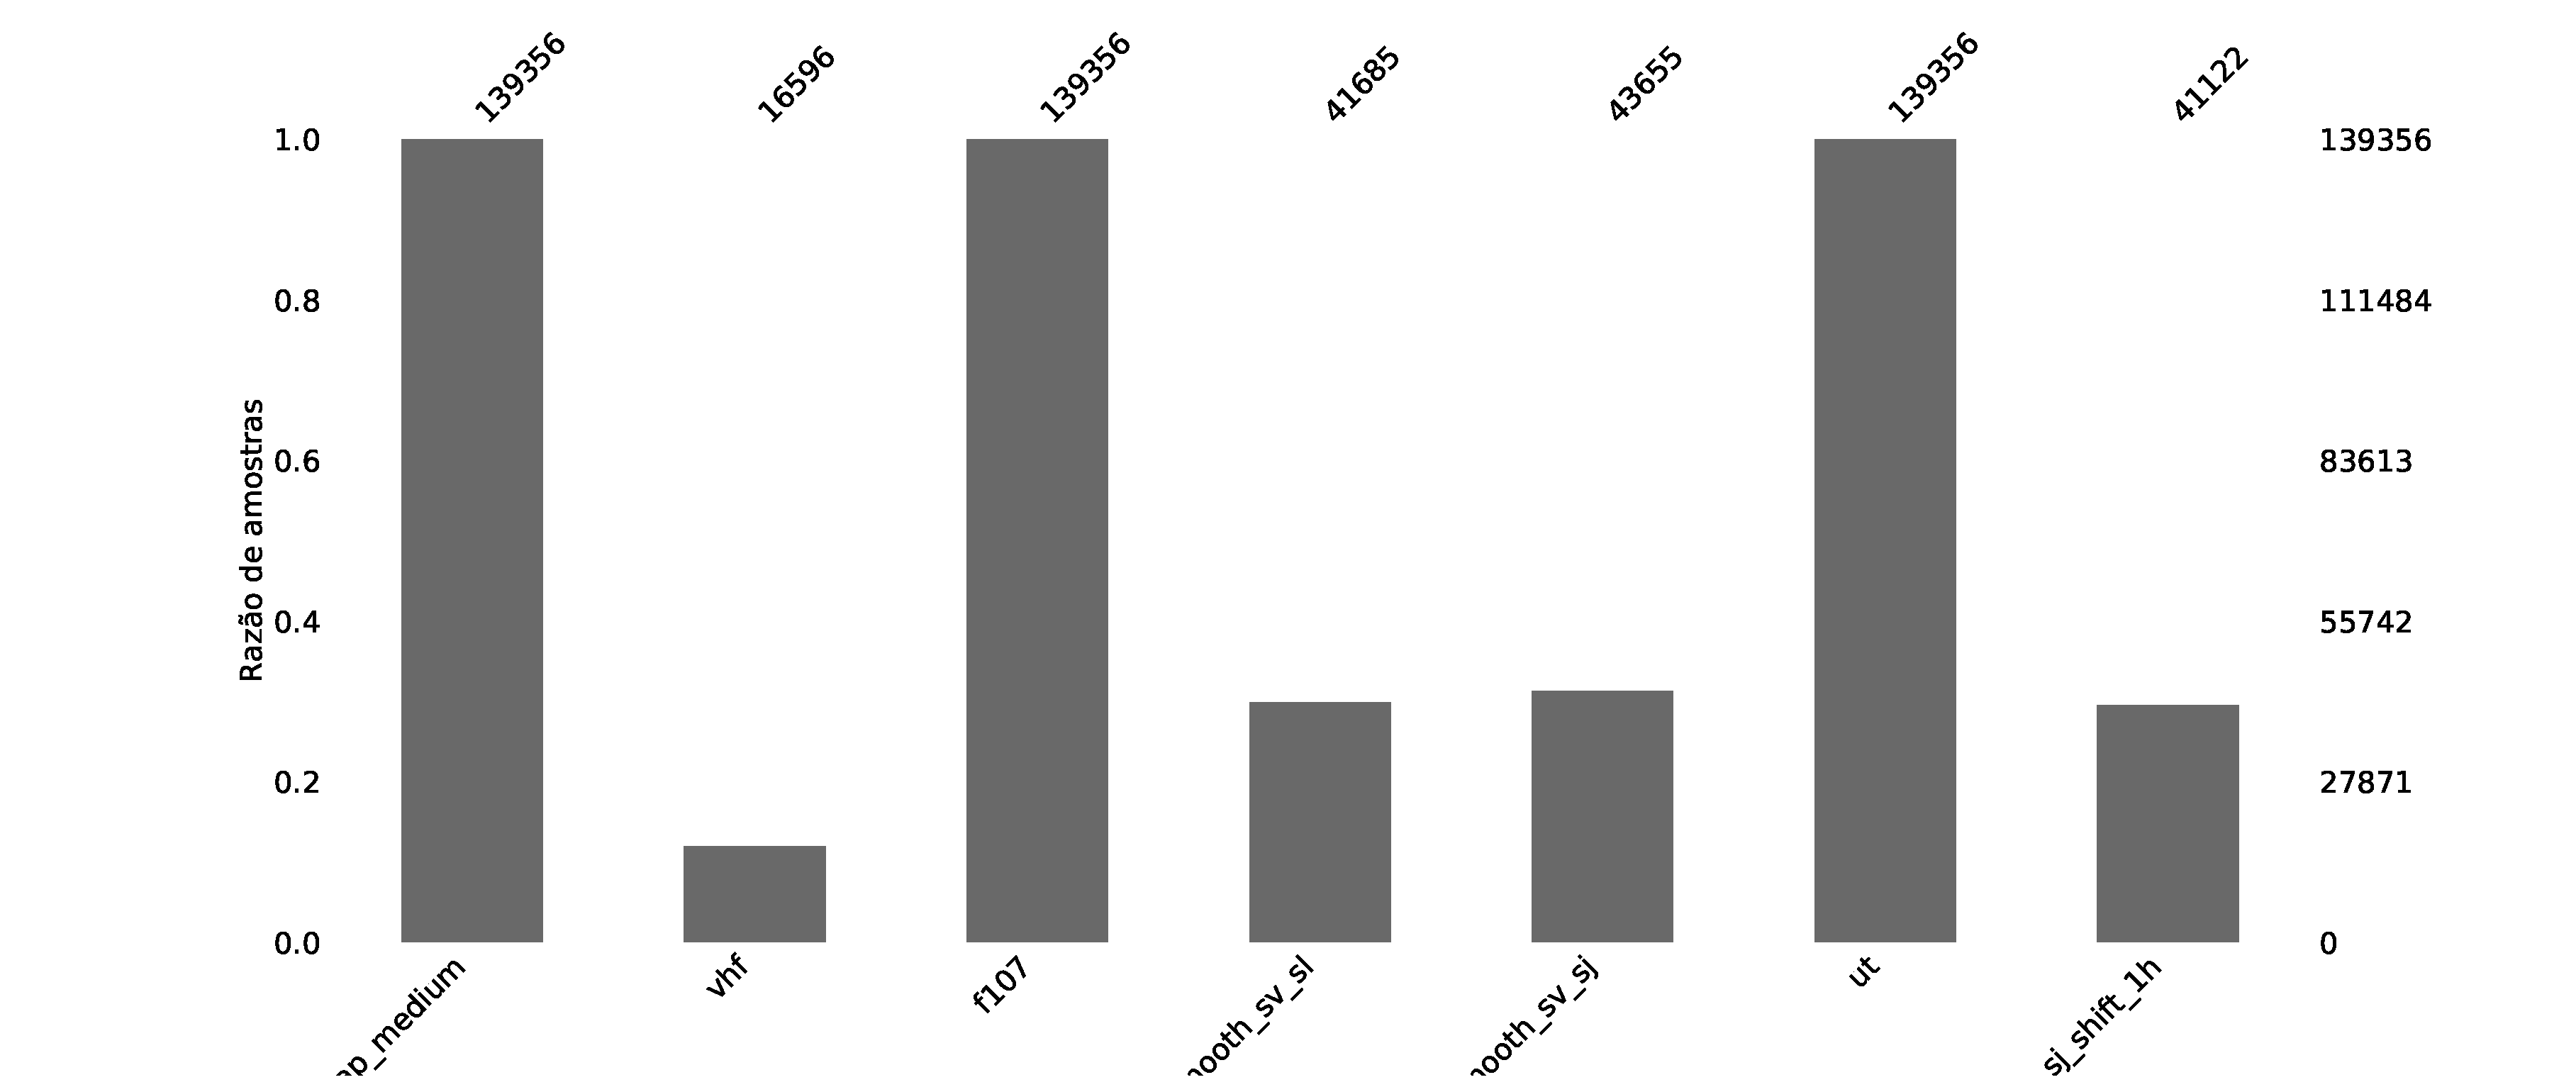
\includegraphics[width=1.2\linewidth]{./Figuras/results-original/nulltotal.eps}}
\caption{Razão e total de dados não nulos por atributo. Fonte: próprio autor.}
\label{fig:nulltotal}
\end{figure}

As variáveis adotadas podem ser agrupados pelo termo conjunto original, e elas são:

\begin{itemize}
\item {\bf ut} representa a hora em São Luiz em minutos, em intervalos de 5 minutos;
\item {\bf vhf} é a velocidade máxima de deriva vertical do plasma medida em São Luiz entre as 17-18 LT (20-21 UT), com resolução de um valor por dia;
\item {\bf ap\_medium} é a média do índice ap definido por:
\begin{equation}\label{eq:ap}
\sum_{i=1}^{n}\sum_{j=1}^{i}\frac{ap_{j}}{ni}\mbox{,}~
\end{equation}
onde $ap_1$ corresponde à ap15\_18ut, $ap_2$ à ap12\_15ut até ap00\_03ut, mais ap21\_00ut e ap18\_21ut do dia anterior, totalizando um intervalo de 24 horas, com $n=8$. Este valor tem resolução diária;
\item {\bf f107} é o fluxo solar, com resolução de uma medida por dia;
\item {\bf s4\_smooth\_sv\_sl} é o maior valor do índice S4 medido em São Luiz, em um período de 5 minutos;
\item {\bf s4\_smooth\_sv\_sj} é o maior valor do índice S4 medido em São José dos Campos, em um período de 5 minutos;
\item {\bf s4\_sj\_shift\_1h} é o S4 estimado com uma hora de antecedência para São José dos Campos, com resolução de 5 minutos.
\end{itemize}

E os cuidados, assim, como os pré-processamentos foram:

\begin{itemize}
\item A adoção do termo São Luiz em relação à equador magnético foi preferida, pois este está em movimento, e ao longo do período coletado, assim como em extensões deste período, não estará no mesmo lugar, enquanto os dados são sempre coletados em uma estação fixa em São Luiz;
\item A adoção do termo São José dos Campos em relação a pico da anomalia ocorre, pois a localização do pico depende da quantidade de radiação emitida pelo Sol em seu regime, ciclo solar. Nos anos de 2000, 2001, 2002, o pico da anomalia estava em São José dos Campos, porém nos anos de 2018 e 2019 este se encontra em Presidente Prudente. Finalmente, os dados foram sempre coletados em uma estação fixa em São José dos Campos;
\item A altura hF não é amostrada em intervalos regulares ao longo do período de dados coletados, inicialmente, ela era amostrada em 15 min, e posteriormente passou a ser amostrado em 10 min, portanto neste trabalho se reamostrou toda a série para o intervalo de 10 min, que foi então interpolado por um spline de grau 3, até um máximo de 10 pontos ausentes na vizinhança do ponto a ser interpolado. Finalmente {\bf vhf} é calculada utilizando a versão de hF preprocessada;
\item Quanto as variáveis definidas em temos do índice $S_4$, primeiro, somente serão aceitas medidas cuja elevação entre a estação e o receptor sejam maiores que 30 graus; segundo todos os dados coletados em uma mesma cidade mas por diferente estações são combinados, de forma a reduzir as lacunas; terceiro, os dados de cintilação apresentam resolução temporal de 1 min, e são coletados para cada satélite acima do plano de horizonte da estação, portanto, existem vários dados por minuto, com objetivo de ficar-se somente com um dado, estes foram agrupados tomando-se o maior valor de cintilação; terceiro, os dados com resolução de um minuto são então interpolados por spline de ordem 3 com limite de quatro valores ausentes; quinto, os dados são suavizados por um filtro de Savitz-Goley centrado de ordem 3 com janela de tamanho 5, o que levaria a necessidade de apenas, 2 amostras de dados futuros; finalmente, os dados são reamostrados para um intervalo de 5 minutos;
\item A adoção de ap em preferência à Kp se deve a esta apresentar uma escala linear e, portanto ser mais condizente com operações como média. A escolha do novo intervalo é realizada, devido ao fato de que a definição original em \cite{REZENDE:2009} não ser clara.
\end{itemize}

Uma abordagem de normalização para o intervalo $[0,05,\,0,95]$ é aplicado a todos os atributos preditores (uma para cada atributo) antes da utilização do algoritmo de aprendizagem de máquina. Este intervalo é adotado já considerando a possibilidade de aplicação de redes neurais com função de ativação sigmoide, haja visto que esta sofre saturação para valores próximos de 0 e 1.

Resta novamente dois elementos a serem definidos, o tipo de problema tratado e por consequência os algoritmos e as métricas a serem utilizadas. Uma que vez que se trata de uma reprodução parcial, o problema de regressão foi considerado, neste caso utilizando a ferramente XGBOOST, que também emprega árvores de decisão e regressão em técnicas de conjunto, neste caso o boosting; as métricas adotadas foram o erro quadrático médio e o erro absoluto máximo, este último sendo capaz de lidar melhor com o desbalanceamento das amostras.

O segundo problema tratado foi o de classificação, e para tal a variável {\bf s4\_sj\_shift\_1h} foi discretizada utilizando a proposta estabelecida por \cite{MUELLA:2008}, mais a adição de uma classe ausente:

\begin{table}[H]
\begin{center}
\begin{tabular}{|c|c|}
\hline
{\bf INTENSIDADE} & {\bf $S_4$} \\ \hline
Saturado          & $S_4 > 1,0$ \\ \hline
Forte             & $0,6 \le S_4 \le 1,0$ \\ \hline
Moderado          & $0,4 \le S_4 \le 0,6$ \\ \hline
Fraco             & $0,2 \le S_4 \le 0,4$ \\ \hline
Ausente           & $ S_4 \le 0,2 $ \\ \hline
\end{tabular}
\end{center}
\end{table}

Neste caso, tem-se um problema com 5 classes não balanceado e uma abordagem de reasmotragem foi empregada de modo balancear o números de elementos tal que todos estejam próximos da cardinalidade da classe com o maior número de elementos. Esta etapa é realizada após a normalização, e o algoritmo empregado foi o ADASYN. Finalmente, adotou-se como métrica a precisão balanceada, e a ferramenta utilizada também foi o XGBOOST.

\subsection{Metodologia}

Para todos os modelos duas formas de avaliação dos modelos gerados foram empregadas: validação cruzada com 10 subconjuntos e validação com separação no tempo. A primeira consistiu em dividir o conjunto de dados de maneira aleatória (e tal que cada conjunto tivesse a mesma proporção em termos de classes, quando de um problema de classificação) em 10 subconjuntos, e então treinar 10 instâncias do modelo utilizando 9 destes conjuntos, enquanto o conjunto restante foi utilizado para avaliar o modelo. Note que para o $i$-ésimo modelo deve ser excluir o $i$-ésimo subconjunto. Os resultados obtidos então, por cada um dos modelos, são agrupados por uma operação de média aritmética. A segunda abordagem consistiu em particionar o conjunto de dados ordenados no tempo em um ponto $t$, tal que o primeira partição fosse empregada no treinamento de um modelo e a segunda para a avaliação do mesmo.

No caso dos problemas tratados, considerando a validação com separação no tempo, a primeira partição terá aproximadamente 65\% de todos os valores tratados, e consequentemente a segunda partição terá 45\%. O total de amostras é de 1742, das quais então, 958 correspondem a primeira partição e 784 correspondem a segunda partição.

%%%%%%%%%%%%%%%%%%%%%%%%%%%%%%%%%%%%%%%%%%%%%%%%%%%%%%%%%%%%%%%%%%%%%%%%%%%%%%%%%%%%%%%%%%%%%%%%%%%%%%%
%%%%%%%%%%%%%%%%%%%%%%%%%%%%%%%%%%%%%%%%%%%%%%%%%%%%%%%%%%%%%%%%%%%%%%%%%%%%%%%%%%%%%%%%%%%%%%%%%%%%%%%

\subsection{Resultados: Regressão}

A Tabela \ref{tab:results_reg} apresenta as métricas para os resultados obtidos para as duas abordagens de validação. Enquanto, a Figura \ref{fig:rego} apresenta a importância das variáveis segundo o XGBOOST.

\begin{table}[h]
\begin{center}
\begin{tabular}{|c|c|c|}
\hline
Tipo de Validação & mse       & mae   \\ \hline
Validação Cruzada                   & 0,018   & 0,753  \\ \hline
Validação com Separação no Tempo    & 0,016   & 0,553  \\ \hline
\end{tabular}
\end{center}
\vspace{12pt}
\caption{Resultados para a regressão. Fonte: Próprio autor.}
\label{tab:results_reg}
\end{table}

\begin{figure}[h]
\center
\makebox[\textwidth][c]{
\subfigure[fig:rego1][Validação cruzada com 10 subconjuntos.]{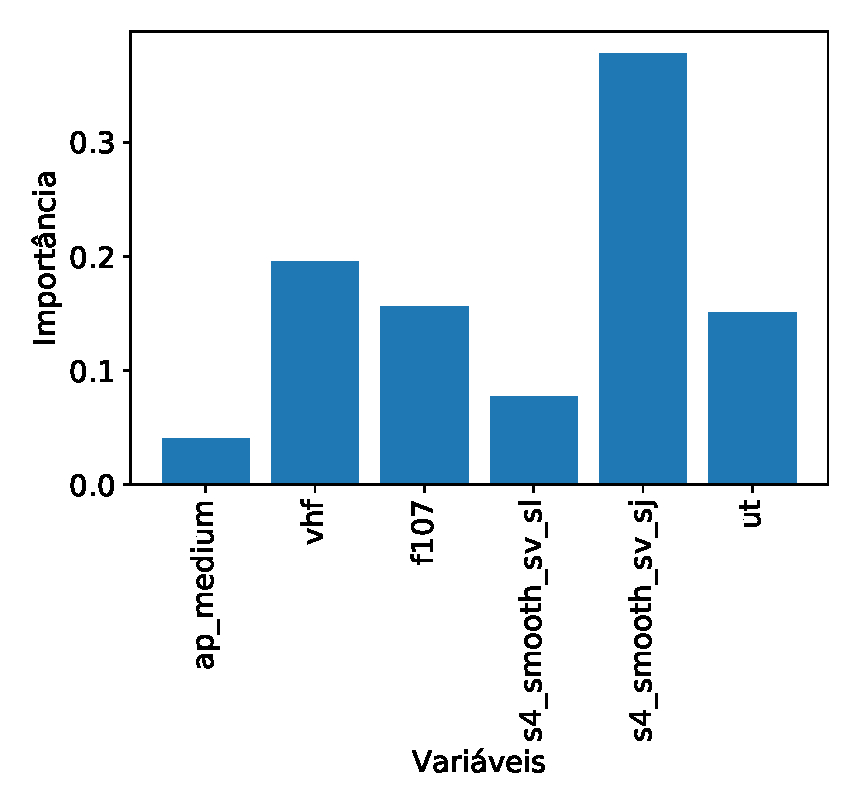
\includegraphics[width=9.5cm]{./Figuras/results-original/regression_kfold_original_958_1742_importance.eps}}
\,\,
\subfigure[fig:rego2][Validação com separação no tempo.]{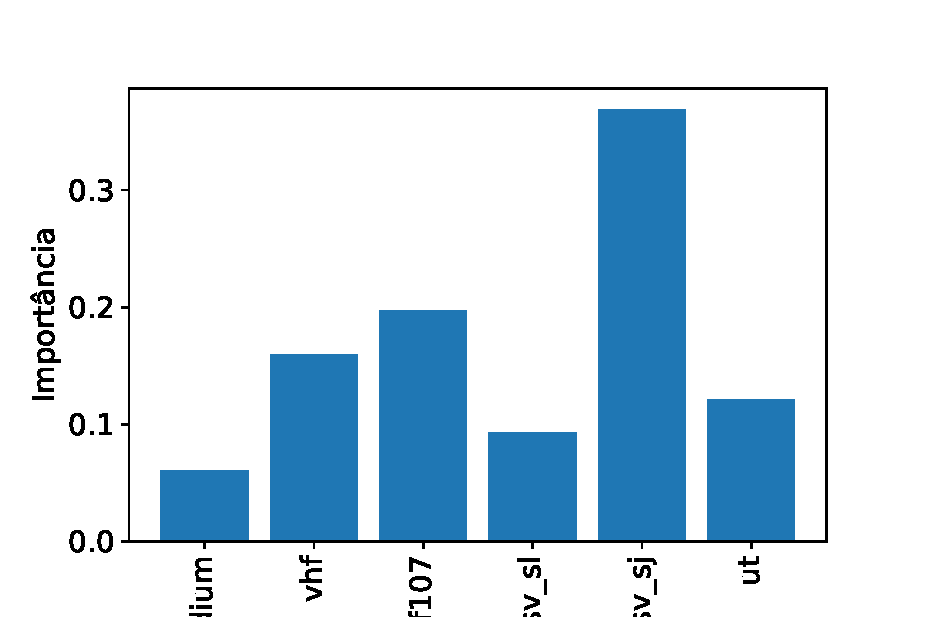
\includegraphics[width=9.5cm]{./Figuras/results-original/regression_intime_original_958_1742_importance.eps}}
}
\caption{Importância de cada atributo segundo XGBOOST. Fonte: próprio autor.}\label{fig:rego}
\end{figure}


\subsection{Resultados: Classificação}

A Tabela \ref{tab:results_class} apresenta as métricas para os resultados obtidos para as duas abordagens de validação. As Figuras \ref{fig:classomik} e \ref{fig:classomii} apresentam respectivamente a matriz de confusão e um gráfico de barras com a importância das variáveis segundo o XGBOOST, para a validação cruzada e a validação com separação no tempo.

\begin{table}[h]
\begin{center}
\begin{tabular}{|c|c|}
\hline
Tipo de Validação & precisão balanceada   \\ \hline
Validação Cruzada                   & 0,651    \\ \hline
Validação com Separação no Tempo    & 0,363     \\ \hline
\end{tabular}
\end{center}
\vspace{12pt}
\caption{Resultados para a classificação. Fonte: Próprio autor.}
\label{tab:results_class}
\end{table}

\begin{figure}[h]
\center
\makebox[\textwidth][c]
{
\subfigure[fig:classomk1][Matriz de Confusão.]{\includegraphics[width=11.5cm]{./Figuras/results-original/classification_kfold_original_958_1742_confusion_matrix.eps}}
\,\,
\subfigure[fig:classoik2][Importância dos atributos segundo XGBOOST.]{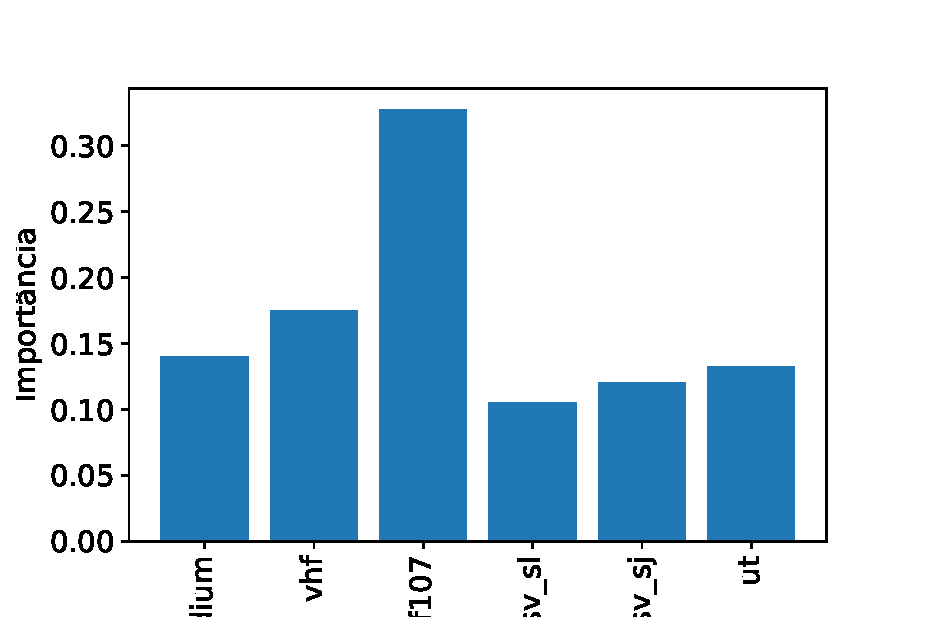
\includegraphics[width=9.5cm]{./Figuras/results-original/classification_kfold_original_958_1742_importance.eps}}
}
\caption{Resultados para o problema de classificação utilizando de validação cruzada com 10 subconjuntos. Fonte: próprio autor.}
\label{fig:classomik}
\end{figure}

\begin{figure}[h]
\center
\makebox[\textwidth][c]
{
\subfigure[fig:classoii1][Matriz de Confusão.]{\includegraphics[width=11.5cm]{./Figuras/results-original/classification_intime_original_958_1742_confusion_matrix.eps}}
\,\,
\subfigure[fig:classoii2][Importância dos atributos segundo XGBOOST.]{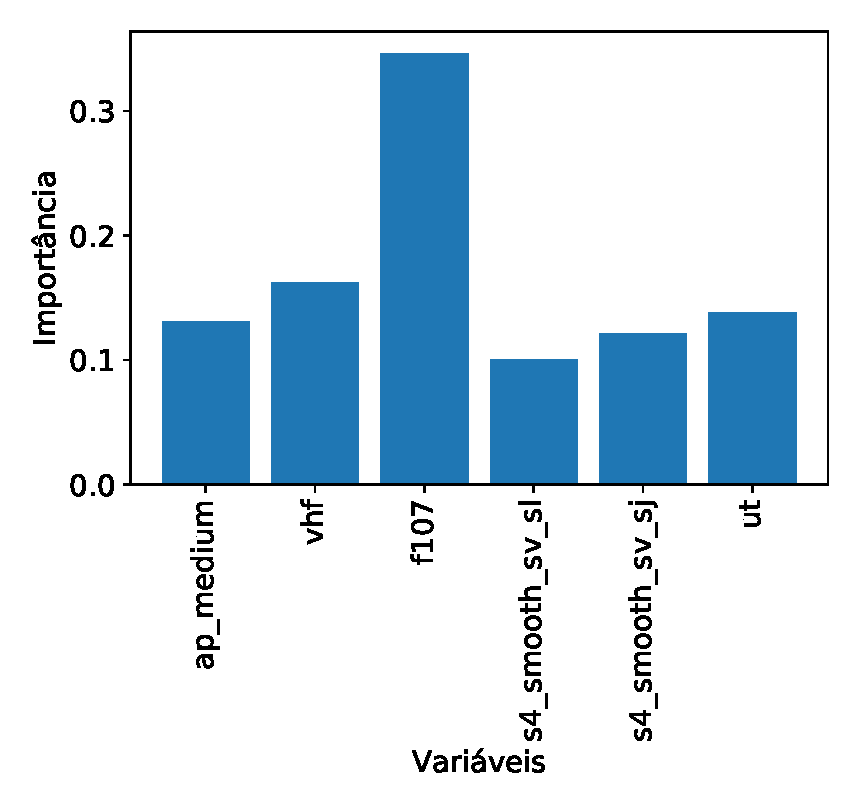
\includegraphics[width=9.5cm]{./Figuras/results-original/classification_intime_original_958_1742_importance.eps}}
}
\caption{Resultados para o problema de classificação utilizando de validação com separação no tempo. Fonte: próprio autor.}
\label{fig:classomii}
\end{figure}

\section{Novos atributos}

%%%%%%%%%%%%%%%%%%%%%%%%%%%%%%%%%%%%%%%%%%%%%%%%%%%%%%%%%%%%%%%%%%%%%%%%%%%%%%%%%%%%%%%%%%%%%%%%%%%%%%%
%%%%%%%%%%%%%%%%%%%%%%%%%%%%%%%%%%%%%%%%%%%%%%%%%%%%%%%%%%%%%%%%%%%%%%%%%%%%%%%%%%%%%%%%%%%%%%%%%%%%%%%

\subsection{Conjunto v1}\label{sec:v1}

A primeira versão após a reprodução foi gerada redefinindo variáveis e adicionando novas. Partindo do conjunto de variáveis original definido na seção \ref{se:rep} as seguintes alterações foram empregadas:

\begin{itemize}
\item Agora, somente serão aceitas variáveis de $S_4$ com valores de elevação acima de 45 graus. E, antes do processo de combinação das amostras para a geração de um único dado por minuto, o valor de S4 é projetado na vertical segundo seu angulo de elevação por:
\begin{equation}
{S_4}_{proj}=S_4[\sin\theta]^{0,9}\mbox{,}~
\end{equation}
onde $\theta$ denota o angulo de elevação;
\item A variável {\bf hf} é a altura inferior da camada F. Tem resolução temporal de 10 min e vai corresponder ao instante da amostra tal que valores para os minutos da forma 5, 15, 25 serão aproximados pelos valores no instante anterior, isto é, 0, 10, 20, por exemplo;
\item A variável {\bf vhf} passa a ter resolução temporal de 10 min análoga a definição para {\bf hf};
\item A variável {\bf month} indica o mês em que a amostra foi coletada.
\end{itemize}

As demais variáveis, assim como os procedimentos de pré-processamento não serão alterados. A distribuição dos dados e a ordem de dados nulos para este conjunto é semelhante ao do conjunto original e, portanto, será omitida.

\subsection{Resultados para o conjunto v1}

A mesma metodologia é utilizada, ou seja, serão utilizadas de validação cruzada e validação com separação no tempo. Entretanto, para o conjunto v1 se tem 1635 amostras, dos quais 899 irão compor a primeira partição.

Os mesmos tipos de modelos e ferramentas são empregadas. A Tabela \ref{tab:results_v1_reg} apresenta as métricas para os resultados obtidos para as duas abordagens de validação. Enquanto, a Figura \ref{fig:regv1} apresenta a importância das variáveis segundo o XGBOOST.

Fica evidente comparando as Tabelas \ref{tab:results_v1_reg} e \ref{tab:results_reg} a melhora dos resultados de regressão quando da nova abordagem de preprocessamento para o $S_4$ e o hF e, portanto, para as suas variáveis associadas, assim como da nova resolução temporal para {\bf vhf} e a adição da variável {\bf hf}.

\begin{table}[h]
\begin{center}
\begin{tabular}{|c|c|c|}
\hline
Tipo de Validação & mse       & mae   \\ \hline
Validação Cruzada                   & 0,013   & 0,706  \\ \hline
Validação com Separação no Tempo    & 0,011   & 0,250  \\ \hline
\end{tabular}
\end{center}
\vspace{12pt}
\caption{Resultados para a regressão. Fonte: Próprio autor.}
\label{tab:results_v1_reg}
\end{table}

\begin{figure}[h]
\center
\makebox[\textwidth][c]{
\subfigure[fig:regv11][Validação cruzada com 10 subconjuntos.]{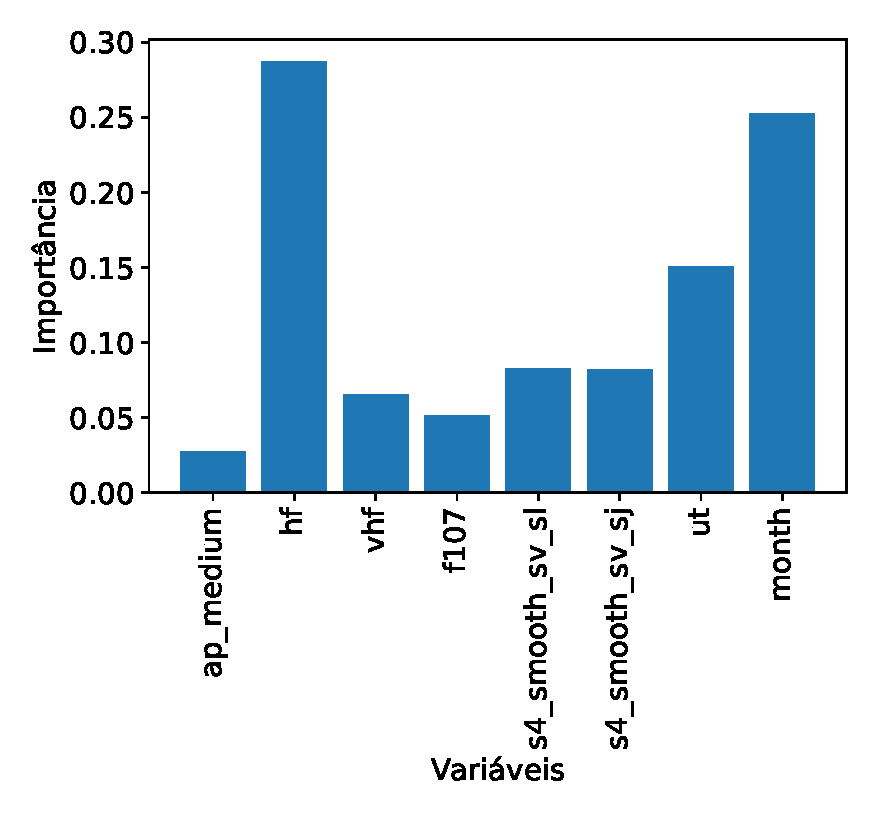
\includegraphics[width=9.5cm]{./Figuras/results-v1/regression_kfold_v1_899_1635_importance.eps}}
\,\,
\subfigure[fig:regv12][Validação com separação no tempo.]{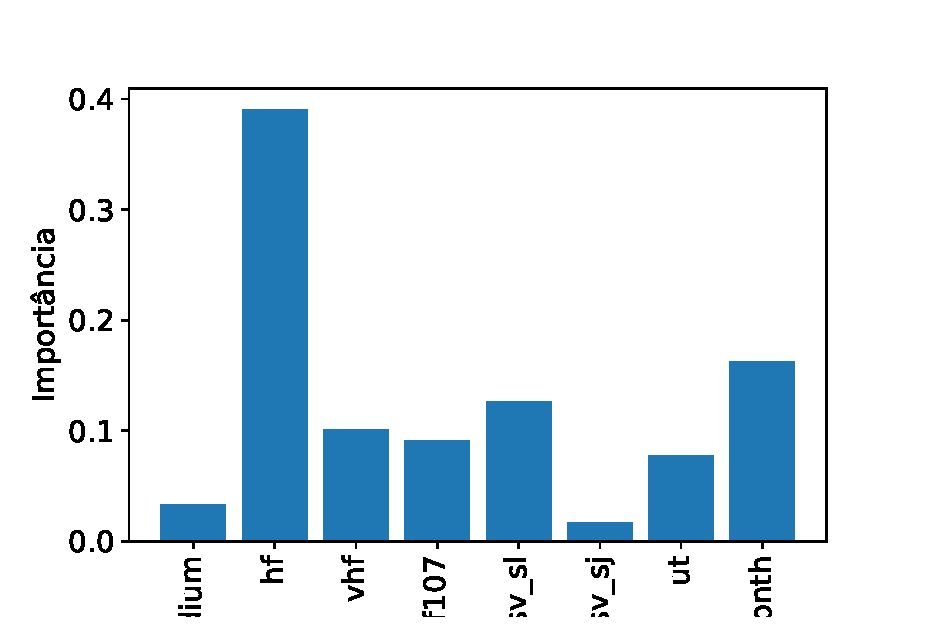
\includegraphics[width=9.5cm]{./Figuras/results-v1/regression_intime_v1_899_1635_importance.eps}}
}
\caption{Importância de cada atributo segundo XGBOOST. Fonte: próprio autor.}\label{fig:regv1}
\end{figure}

A Tabela \ref{tab:results_v1_class} apresenta as métricas para os resultados obtidos para as duas abordagens de validação. As Figuras \ref{fig:classv1mik} e \ref{fig:classv1mii} apresentam respectivamente a matriz de confusão e um gráfico de barras com a importância das variáveis segundo o XGBOOST, para a validação cruzada e a validação com separação no tempo.

\begin{table}[h]
\begin{center}
\begin{tabular}{|c|c|}
\hline
Tipo de Validação & precisão balanceada   \\ \hline
Validação Cruzada                   & 0,571    \\ \hline
Validação com Separação no Tempo    & 0,472     \\ \hline
\end{tabular}
\end{center}
\vspace{12pt}
\caption{Resultados para a classificação. Fonte: Próprio autor.}
\label{tab:results_v1_class}
\end{table}

Quando comparando as Tabelas \ref{tab:results_v1_class} e \ref{tab:results_class} que fornecem respectivamente os resultados para o conjunto de atributos v1 e o conjunto original, tem-se que para o problema de classificação houve uma piora dos resultados quando considerado validação cruzada, e uma melhora quando considerado validação com separação no tempo. Todavia, fica claro que o número de amostras não é suficiente para modelar corretamente as distribuições e, assim, resultados melhores ou piores de mesma ordem não permitem concluir se um resultado é ou não melhor. Tal fato irá se manifestar em todos os resultados obtidos nesta proposta. Note também, que a comparação entre os conjuntos original e v1 devem ser feitas com olhar rigoroso e indireto, pois as variáveis respostas são ligeiramente diferentes, devido ao preprocessamento. Contudo é clara a necessidade da redefinição da variável reposta haja visto o conhecimento especialista \cite{MUELLA:2008}.

\begin{figure}[h]
\center
\makebox[\textwidth][c]
{
\subfigure[fig:classv1mk1][Matriz de Confusão.]{\includegraphics[width=11.5cm]{./Figuras/results-v1/classification_kfold_v1_899_1635_confusion_matrix.eps}}
\,\,
\subfigure[fig:classv1ik2][Importância dos atributos segundo XGBOOST.]{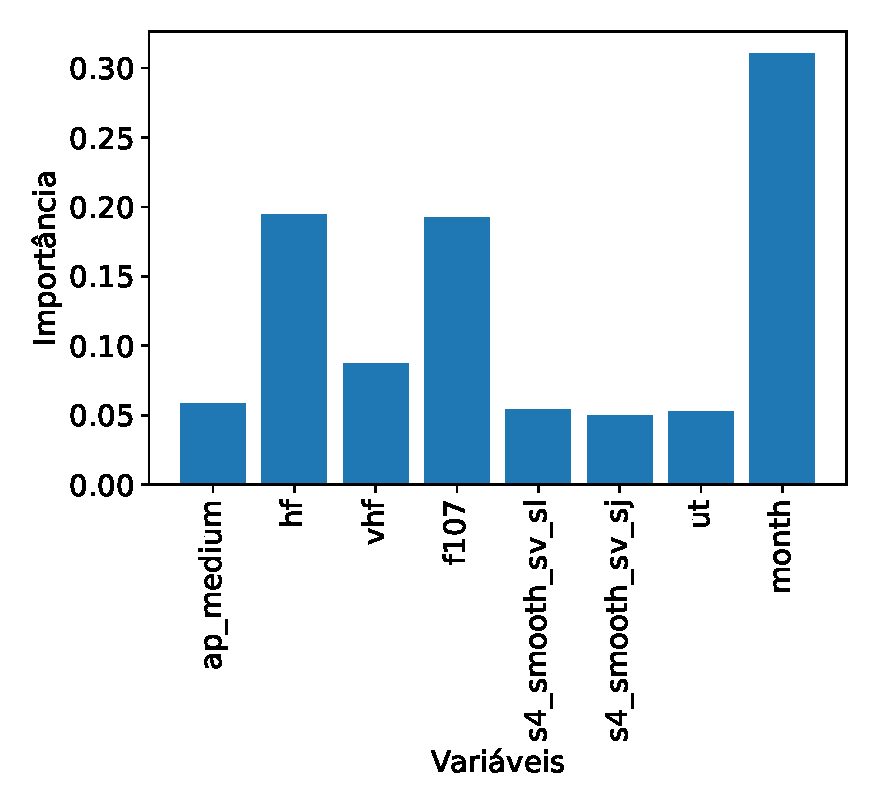
\includegraphics[width=9.5cm]{./Figuras/results-v1/classification_kfold_v1_899_1635_importance.eps}}
}
\caption{Resultados para o problema de classificação utilizando de validação cruzada com 10 subconjuntos. Fonte: próprio autor.}
\label{fig:classv1mik}
\end{figure}

\begin{figure}[h]
\center
\makebox[\textwidth][c]
{
\subfigure[fig:classv1ii1][Matriz de Confusão.]{\includegraphics[width=11.5cm]{./Figuras/results-v1/classification_intime_v1_899_1635_confusion_matrix.eps}}
\,\,
\subfigure[fig:classv1ii2][Importância dos atributos segundo XGBOOST.]{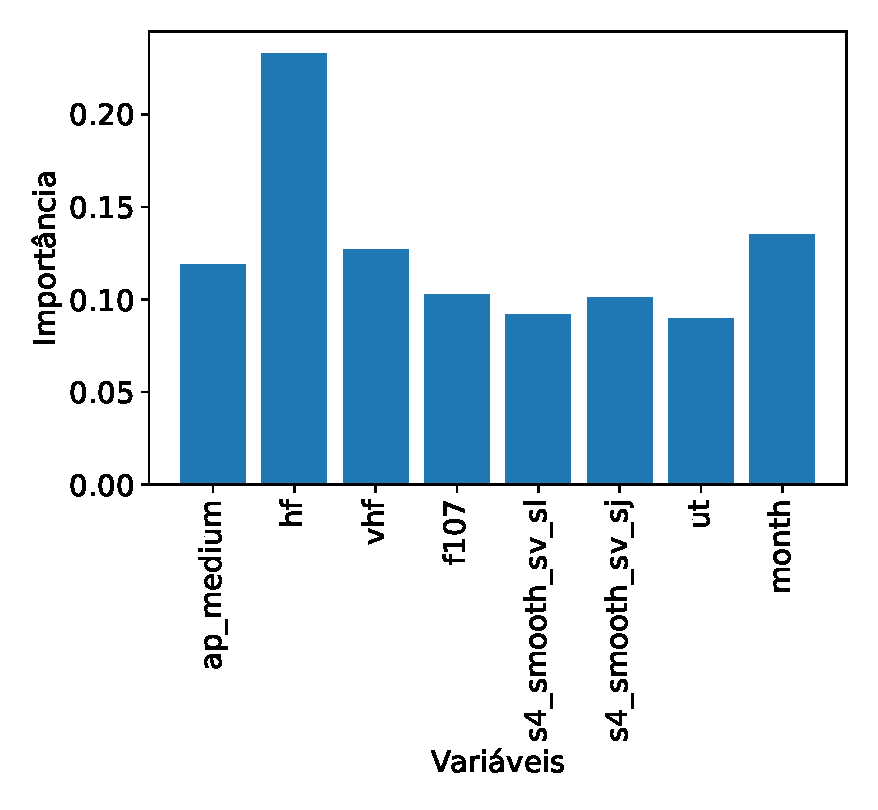
\includegraphics[width=9.5cm]{./Figuras/results-v1/classification_intime_v1_899_1635_importance.eps}}
}
\caption{Resultados para o problema de classificação utilizando de validação com separação no tempo. Fonte: próprio autor.}
\label{fig:classv1mii}
\end{figure}

%%%%%%%%%%%%%%%%%%%%%%%%%%%%%%%%%%%%%%%%%%%%%%%%%%%%%%%%%%%%%%%%%%%%%%%%%%%%%%%%%%%%%%%%%%%%%%%%%%%%%%%
%%%%%%%%%%%%%%%%%%%%%%%%%%%%%%%%%%%%%%%%%%%%%%%%%%%%%%%%%%%%%%%%%%%%%%%%%%%%%%%%%%%%%%%%%%%%%%%%%%%%%%%

\subsection{Conjunto v1 sem dados de cintilação em São Luiz: resultados}

O conjunto de atributos preditores usado aqui é inicialmente o mesmo empregado na seção \ref{sec:v1}, isto é, o conjunto v1, porém neste contexto se descarta a contribuição $S_4$ referente a São Luiz, ou seja, a variável {\bf s4\_smooth\_sv\_sl}. O número total de amostras para esta abordagem é de 4778, onde no processo de validação com separação no tempo 2627 amostras são utilizadas para a fase de treinamento, enquanto 2151 amostras foram utilizadas para validação. A Tabela \ref{tab:results_v1_w_reg} apresenta os resultados obtidos para a regressão.

\begin{table}[h]
\begin{center}
\begin{tabular}{|c|c|c|}
\hline
Tipo de Validação & mse       & mae   \\ \hline
Validação Cruzada                   & 0,013   & 0,780  \\ \hline
Validação com Separação no Tempo    & 0,026   & 0,974  \\ \hline
\end{tabular}
\end{center}
\vspace{12pt}
\caption{Resultados para a regressão. Fonte: Próprio autor.}
\label{tab:results_v1_w_reg}
\end{table}

Comparando às Tabelas \ref{tab:results_v1_w_reg} e \ref{tab:results_v1_reg} fica evidente uma piora dos resultados devido ao descarte de dados de cintilação em São Luiz, porém tal fato é mais gritante para validação com separação no tempo, onde o número total de amostras utilizadas para o treinamento é muito pequeno, o que destaca a necessidade de aumentar a base de dados. Resultado semelhante é encontrado no problema de classificação comparando as tabelas \ref{tab:results_v1_w_class} e \ref{tab:results_v1_class}.

\begin{figure}[h]
\center
\makebox[\textwidth][c]{
\subfigure[fig:regv1w1][Validação cruzada com 10 subconjuntos.]{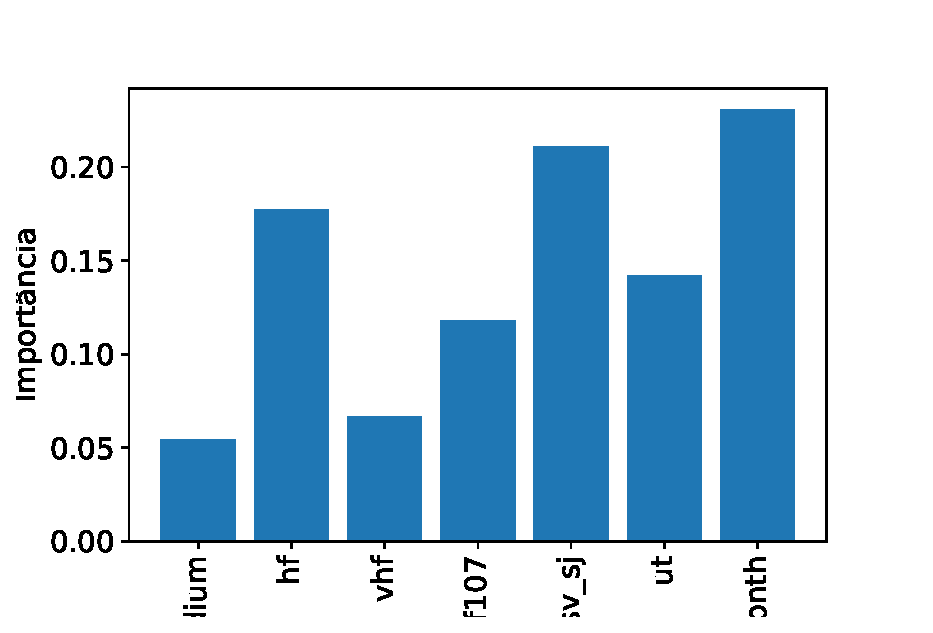
\includegraphics[width=9.5cm]{./Figuras/results-v1/regression_kfold_v1-without-sl_2627_4778_importance.eps}}
\,\,
\subfigure[fig:regv1w2][Validação com separação no tempo.]{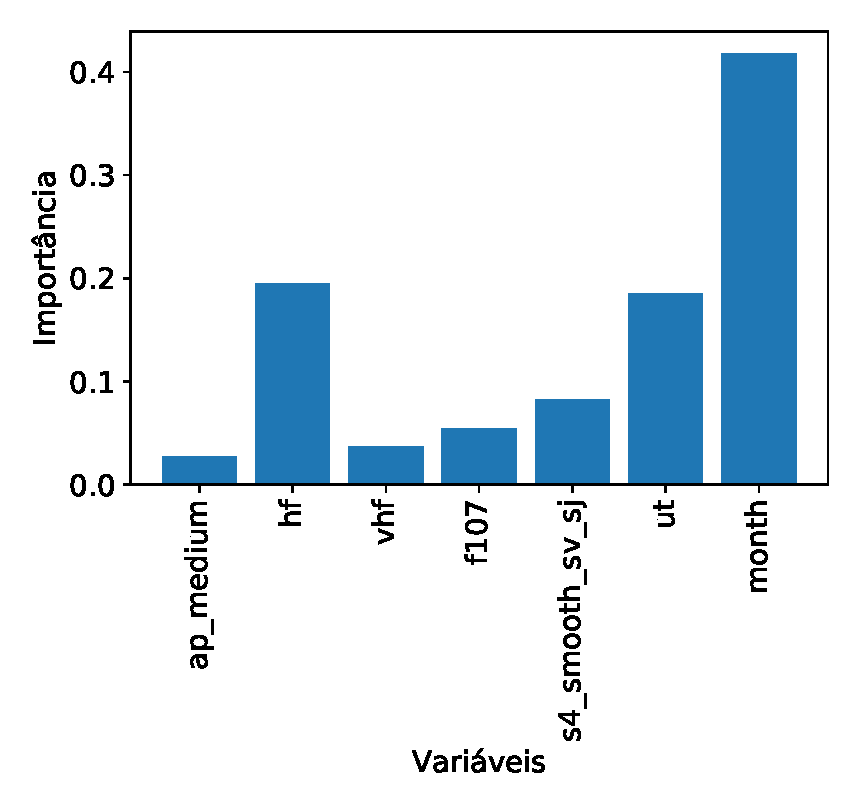
\includegraphics[width=9.5cm]{./Figuras/results-v1/regression_intime_v1-without-sl_2627_4778_importance.eps}}
}
\caption{Importância de cada atributo segundo XGBOOST. Fonte: próprio autor.}\label{fig:regv1w}
\end{figure}

A Tabela \ref{tab:results_v1_w_class} apresenta as métricas para as duas abordagens de validação no contexto do problema de classificação. As Figuras \ref{fig:classv1wmik} e \ref{fig:classv1wmii} apresentam respectivamente a matriz de confusão e um gráfico de barras com a importância das variáveis segundo o XGBOOST, para a validação cruzada e a validação com separação no tempo.

\begin{table}[h]
\begin{center}
\begin{tabular}{|c|c|}
\hline
Tipo de Validação & precisão balanceada   \\ \hline
Validação Cruzada                   & 0,463    \\ \hline
Validação com Separação no Tempo    & 0,248     \\ \hline
\end{tabular}
\end{center}
\vspace{12pt}
\caption{Resultados para a classificação. Fonte: Próprio autor.}
\label{tab:results_v1_w_class}
\end{table}

\begin{figure}[H]
\center
\makebox[\textwidth][c]
{
\subfigure[fig:classv1wmk1][Matriz de Confusão.]{\includegraphics[width=11.5cm]{./Figuras/results-v1/classification_kfold_v1-without-sl_2627_4778_confusion_matrix.eps}}
\,\,
\subfigure[fig:classv1wik2][Importância dos atributos segundo XGBOOST.]{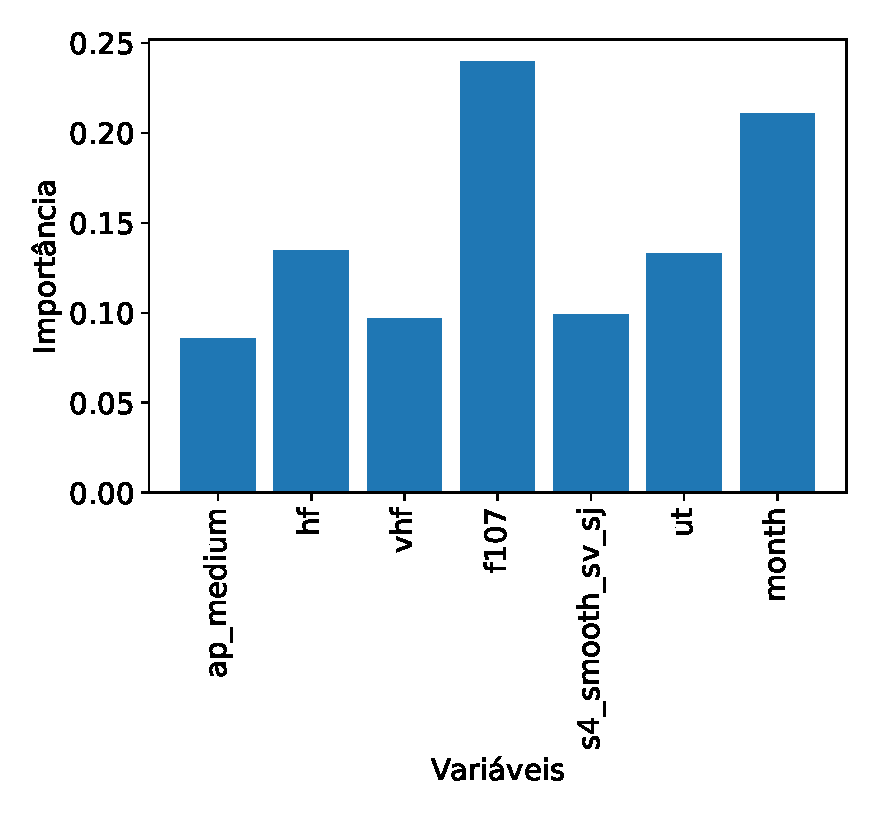
\includegraphics[width=9.5cm]{./Figuras/results-v1/classification_kfold_v1-without-sl_2627_4778_importance.eps}}
}
\caption{Resultados para o problema de classificação utilizando de validação cruzada com 10 subconjuntos. Fonte: próprio autor.}
\label{fig:classv1wmik}
\end{figure}

\begin{figure}[H]
\center
\makebox[\textwidth][c]
{
\subfigure[fig:classv1wii1][Matriz de Confusão.]{\includegraphics[width=11.5cm]{./Figuras/results-v1/classification_intime_v1-without-sl_2627_4778_confusion_matrix.eps}}
\,\,
\subfigure[fig:classv1wii2][Importância dos atributos segundo XGBOOST.]{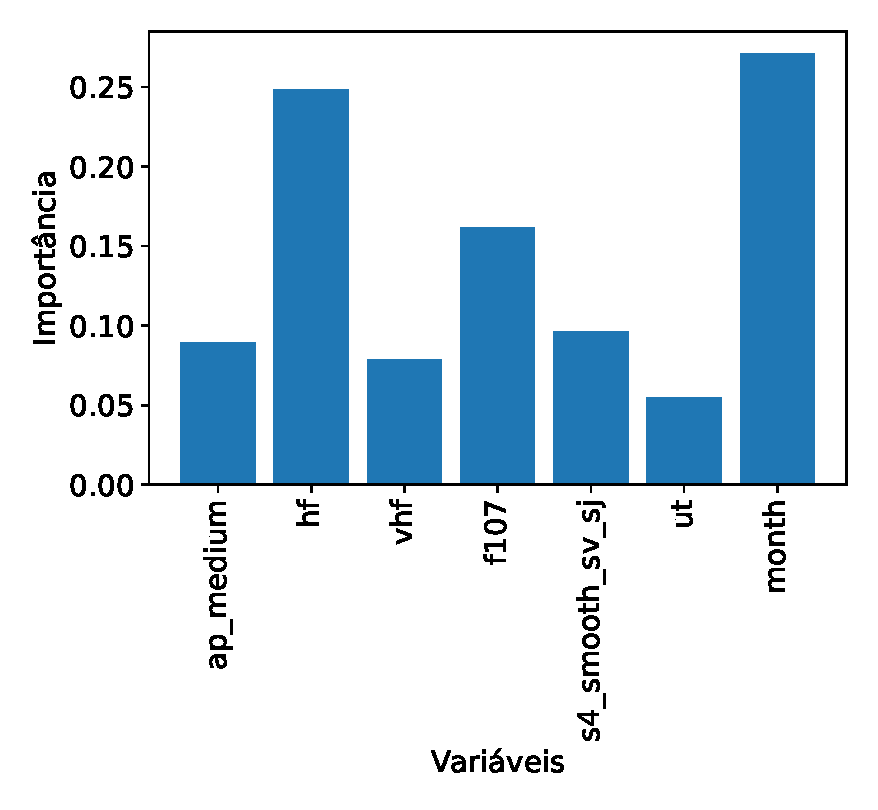
\includegraphics[width=9.5cm]{./Figuras/results-v1/classification_intime_v1-without-sl_2627_4778_importance.eps}}
}
\caption{Resultados para o problema de classificação utilizando de validação com separação no tempo. Fonte: próprio autor.}
\label{fig:classv1wmii}
\end{figure}

De forma geral, os resultados obtidos descartando os dados de $S_4$ de São Luiz são interessantes um vez que abrem possibilidades para novos problemas, um destes é apresentado na próxima seção, apesar de serem relativamente inferiores.

%%%%%%%%%%%%%%%%%%%%%%%%%%%%%%%%%%%%%%%%%%%%%%%%%%%%%%%%%%%%%%%%%%%%%%%%%%%%%%%%%%%%%%%%%%%%%%%%%%%%%%%
%%%%%%%%%%%%%%%%%%%%%%%%%%%%%%%%%%%%%%%%%%%%%%%%%%%%%%%%%%%%%%%%%%%%%%%%%%%%%%%%%%%%%%%%%%%%%%%%%%%%%%%

\section{Previsão de de cintilação ionosférica com 1 h de antecedência ao longo do território brasileiro}

Uma vez descarta a contribuição do índice $S_4$ da estação de São Luiz, na variável {\bf s4\_smooth\_sv\_sl}, tem-se que o modelo só apresenta dependência local no índice $S_4$, o que leva a uma possibilidade de generalização imediata: a previsão de cintilação ionosférica para múltiplas localizações ao longo do território brasileiro. Nesta configuração fica associada uma localização para cada cidade na base de dados, em outras palavras, cidades com múltiplas estações de medida do índice $S_4$ tem suas medidas agrupadas por uma única tupla de localização da forma (longitude, latitude, altura) medidas respectivamente em graus e metros. Este agrupamento é feito de forma a reduzir lacunas no tempo, ou seja, tratar situações onde uma estação funciona para um dado período, enquanto a outra não, e descartar estruturas na cintilação de pequenas escalas. As anomalias na ionosfera se apresentam em múltiplos tamanhos, o que por sua vez produz pertubações em múltiplas escalas, porém atualmente a rede de coleta de dados não apresenta resolução uniforme ao longo do território brasileiro para o tratamento de de pequenas interferências, assim essas devem ser descartadas.

A Tabela \ref{tab:stations} fornece as localizações utilizadas nesta etapa. A cada localização fica associada um identificador formado pela sigla do estado e o nome da cidade e uma tupla no sistema geodético, ou seja, longitude, latitude e altura. A identificação de uma localização é utilizada diretamente para a construção das variáveis preditoras para este problema a serem definidas, porém, nas fases de treinamento e validação propriamente dita elas devem ser substituídas pela seu correspondente numérico, ou seja, o valor no sistema de coordenadas geodético.

\begin{table}[h]
\begin{center}
\begin{tabular}{|l|c|c|c|}
\hline
Identificação           & Longitude & Latitude & Altura \\ \hline
am\_manaus               & -59,98  & -3,10   & 39 \\ \hline
am\_tefe                 & -64,44  & -3,18   & 0 \\ \hline
ba\_ilheus               & -39,10  & -14,47  & 0 \\ \hline
ba\_salvador             & -38,51  & -13,00  & 12 \\ \hline
ce\_fortaleza            & -38,54  & -3,47   & 14 \\ \hline
df\_brasilia             & -47,87  & -15,76  & 1050 \\ \hline
ma\_sao\_luis             & -44,21  & -2,59   & 0 \\ \hline
ma\_imperatriz           & -47,28  & -5,31   & 134 \\ \hline
mg\_inconfidentes        & -46,33  & -22,32  & 864 \\ \hline
mg\_belo\_horizonte       & -43,95  & -19,87  & 858 \\ \hline
ms\_campo\_grande         & -54,61  & -20,50  & 612 \\ \hline
ms\_dourados             & -54,55  & -22,11  & 756 \\ \hline
mt\_alta\_floresta        & -55,90  & -9,90   & 267 \\ \hline
mt\_cuiaba               & -56,07  & -15,55  & 278 \\ \hline
rj\_macae                & -41,79  & -22,82  & 7 \\ \hline
rj\_ae\_galeao            & -43,24  & -22,82  & 20 \\ \hline
rn\_natal                & -35,12  & -5,84   & 0 \\ \hline
ro\_palmas               & -48,31  & -10,20  & 260 \\ \hline
ro\_porto\_velho          & -63,55  & -8,49   & 1130 \\ \hline
rr\_boa\_vista            & -60,70  & 2,83    & 69 \\ \hline
rs\_santa\_maria          & -53,71  & -29,71  & 110 \\ \hline
rs\_porto\_alegre         & -51,12  & -30,07  & 22 \\ \hline
sp\_presidente\_prudente  & -51,41  & -21,12  & 421 \\ \hline
sp\_sao\_jose\_dos\_campos  & -45,86  & -23,21  & 593 \\ \hline
sp\_cachoeira\_paulista   & -45,00  & -22,41  & 580 \\ \hline
sp\_pirassununga         & -47,33  & -21,99  & 625 \\ \hline
sp\_guaratingueta        & -45,22  & -22,79  & 526 \\ \hline
\end{tabular}
\end{center}
\vspace{12pt}
\caption{A identificação de uma localização é dado pelo estado seguido do nome da cidade. Para cada localização ficam associados longitude, latitude, e altura. Fonte: Próprio autor.}
\label{tab:stations}
\end{table}

O seguinte conjunto de variáveis são definidas para a discussão desta generalização:

\begin{itemize}
\item {\bf latitude, longitude} são extraídos dos valores numéricos para uma dada localização, ou seja, em principio ter-se-ia uma amostra de dados da forma (identificação da localização, {\bf ap\_medium}, ...) o qual tem a identificação da localização substituída pelo seu valor numérico, descartando a altura;
\item {\bf ap\_medium} é  média do índice ap definido pela expressão \ref{eq:ap} correspondendo ao mesmo intervalo já adotado: ap15\_18ut, $ap_2$ à ap12\_15ut até ap00\_03ut, mais ap21\_00ut e ap18\_21ut do dia anterior. Este valor tem resolução diária;
\item {\bf vhf\_day} é a velocidade máxima de deriva vertical do plasma medida em São Luiz entre as 17-19 LT (20-22 UT), com resolução de um valor por dia;
\item {\bf hf\_inst} é altura da parte inferior da camada F amostrada em intervalos de 10 min;
\item {\bf vhf\_inst}é a velocidade de deriva vertical do plasma amostrada em intervalos de 10 min;
\item {\bf f107}  é o fluxo solar, com resolução de uma medida por dia;;
\item {\bf s4} é o máximo da projeção vertical do índice $S_4$ com elevações superiores a 45 graus amostrado em intervalos de 5 min, para uma dada localização. Segue o mesmo pré-processamento discutido para a variável {\bf s4\_smooth\_sv\_sj} no conjunto v1;
\item {\bf ut} representa a hora em São Luiz em minutos, em intervalos de 5 minutos;
\item {\bf month} representa o mês em São Luiz em que a amostra foi avaliada;
\end{itemize}

A altura da amostra de dados é descartada, pois é muito menor que o tamanho das estruturas que causam a cintilação, e o número de localizações tratadas não contempla toda a extensão do território, basicamente, é uma variável com valores muito pequenos frente as outras medidas de espaço (latitude e longitude, por exemplo) para este fenômeno com a devida resolução de tratamento.

As variáveis definidas do hF passam pelo mesmo pré-processamento já discutido anteriormente, reamostragem e interpolação spline.

A variável definida pelo índice $S_4$ após o agrupamento por localização apresentado logo acima, passa pelo preprocessamento já tratado para esta variável, reamostragem, interpolação, filtragem (suavização), reamostragem.

As Figuras \ref{fig:distributionall} e \ref{fig:nulltotalall} mostram respectivamente a distribuição dos dados ao longo do conjunto de amostras, e a razão e o total de dados não nulos. O número total de amostras para este problema é menor, pois se restringe ao período de 2013 a 2014, o qual era o único intervalo com dados para múltiplas estações disponíveis em um primeiro momento. O número total de amostras não nulas foi de 4007.

\begin{figure}[H]
\centering
\makebox[\textwidth][c]{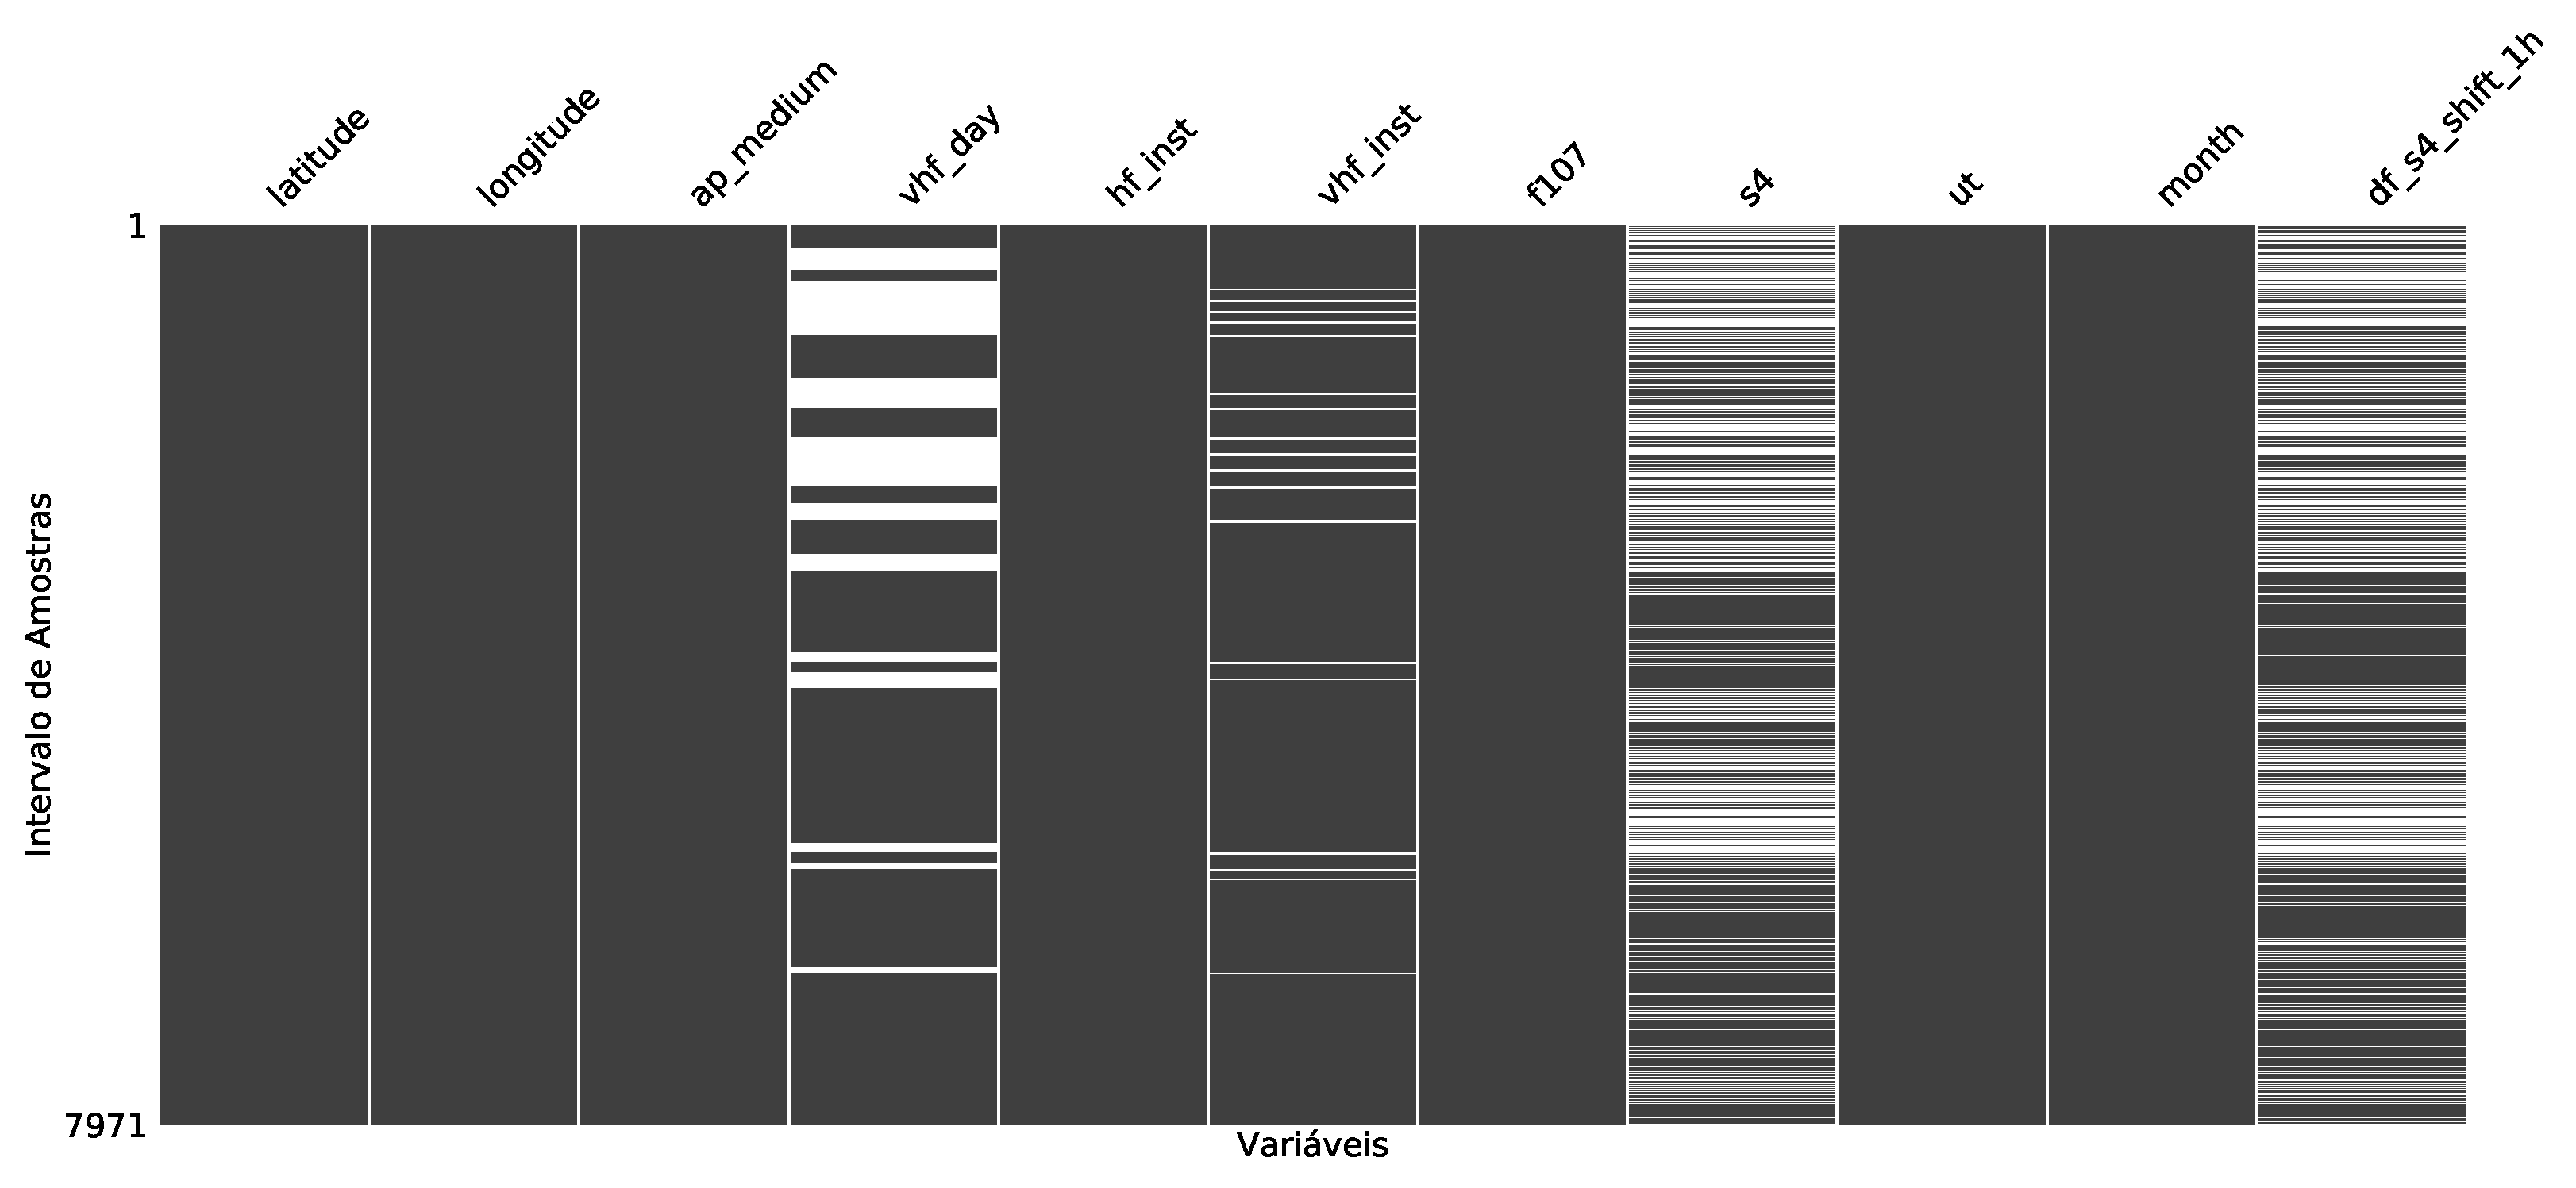
\includegraphics[width=1.2\linewidth]{./Figuras/results-all-stations/distribution.eps}}
\caption{Distribuição dos dados ao longo do conjunto de amostras. Espaços em brancos representam valores ausentes. Fonte: próprio autor.}
\label{fig:distributionall}
\end{figure}

\begin{figure}[H]
\centering
\makebox[\textwidth][c]{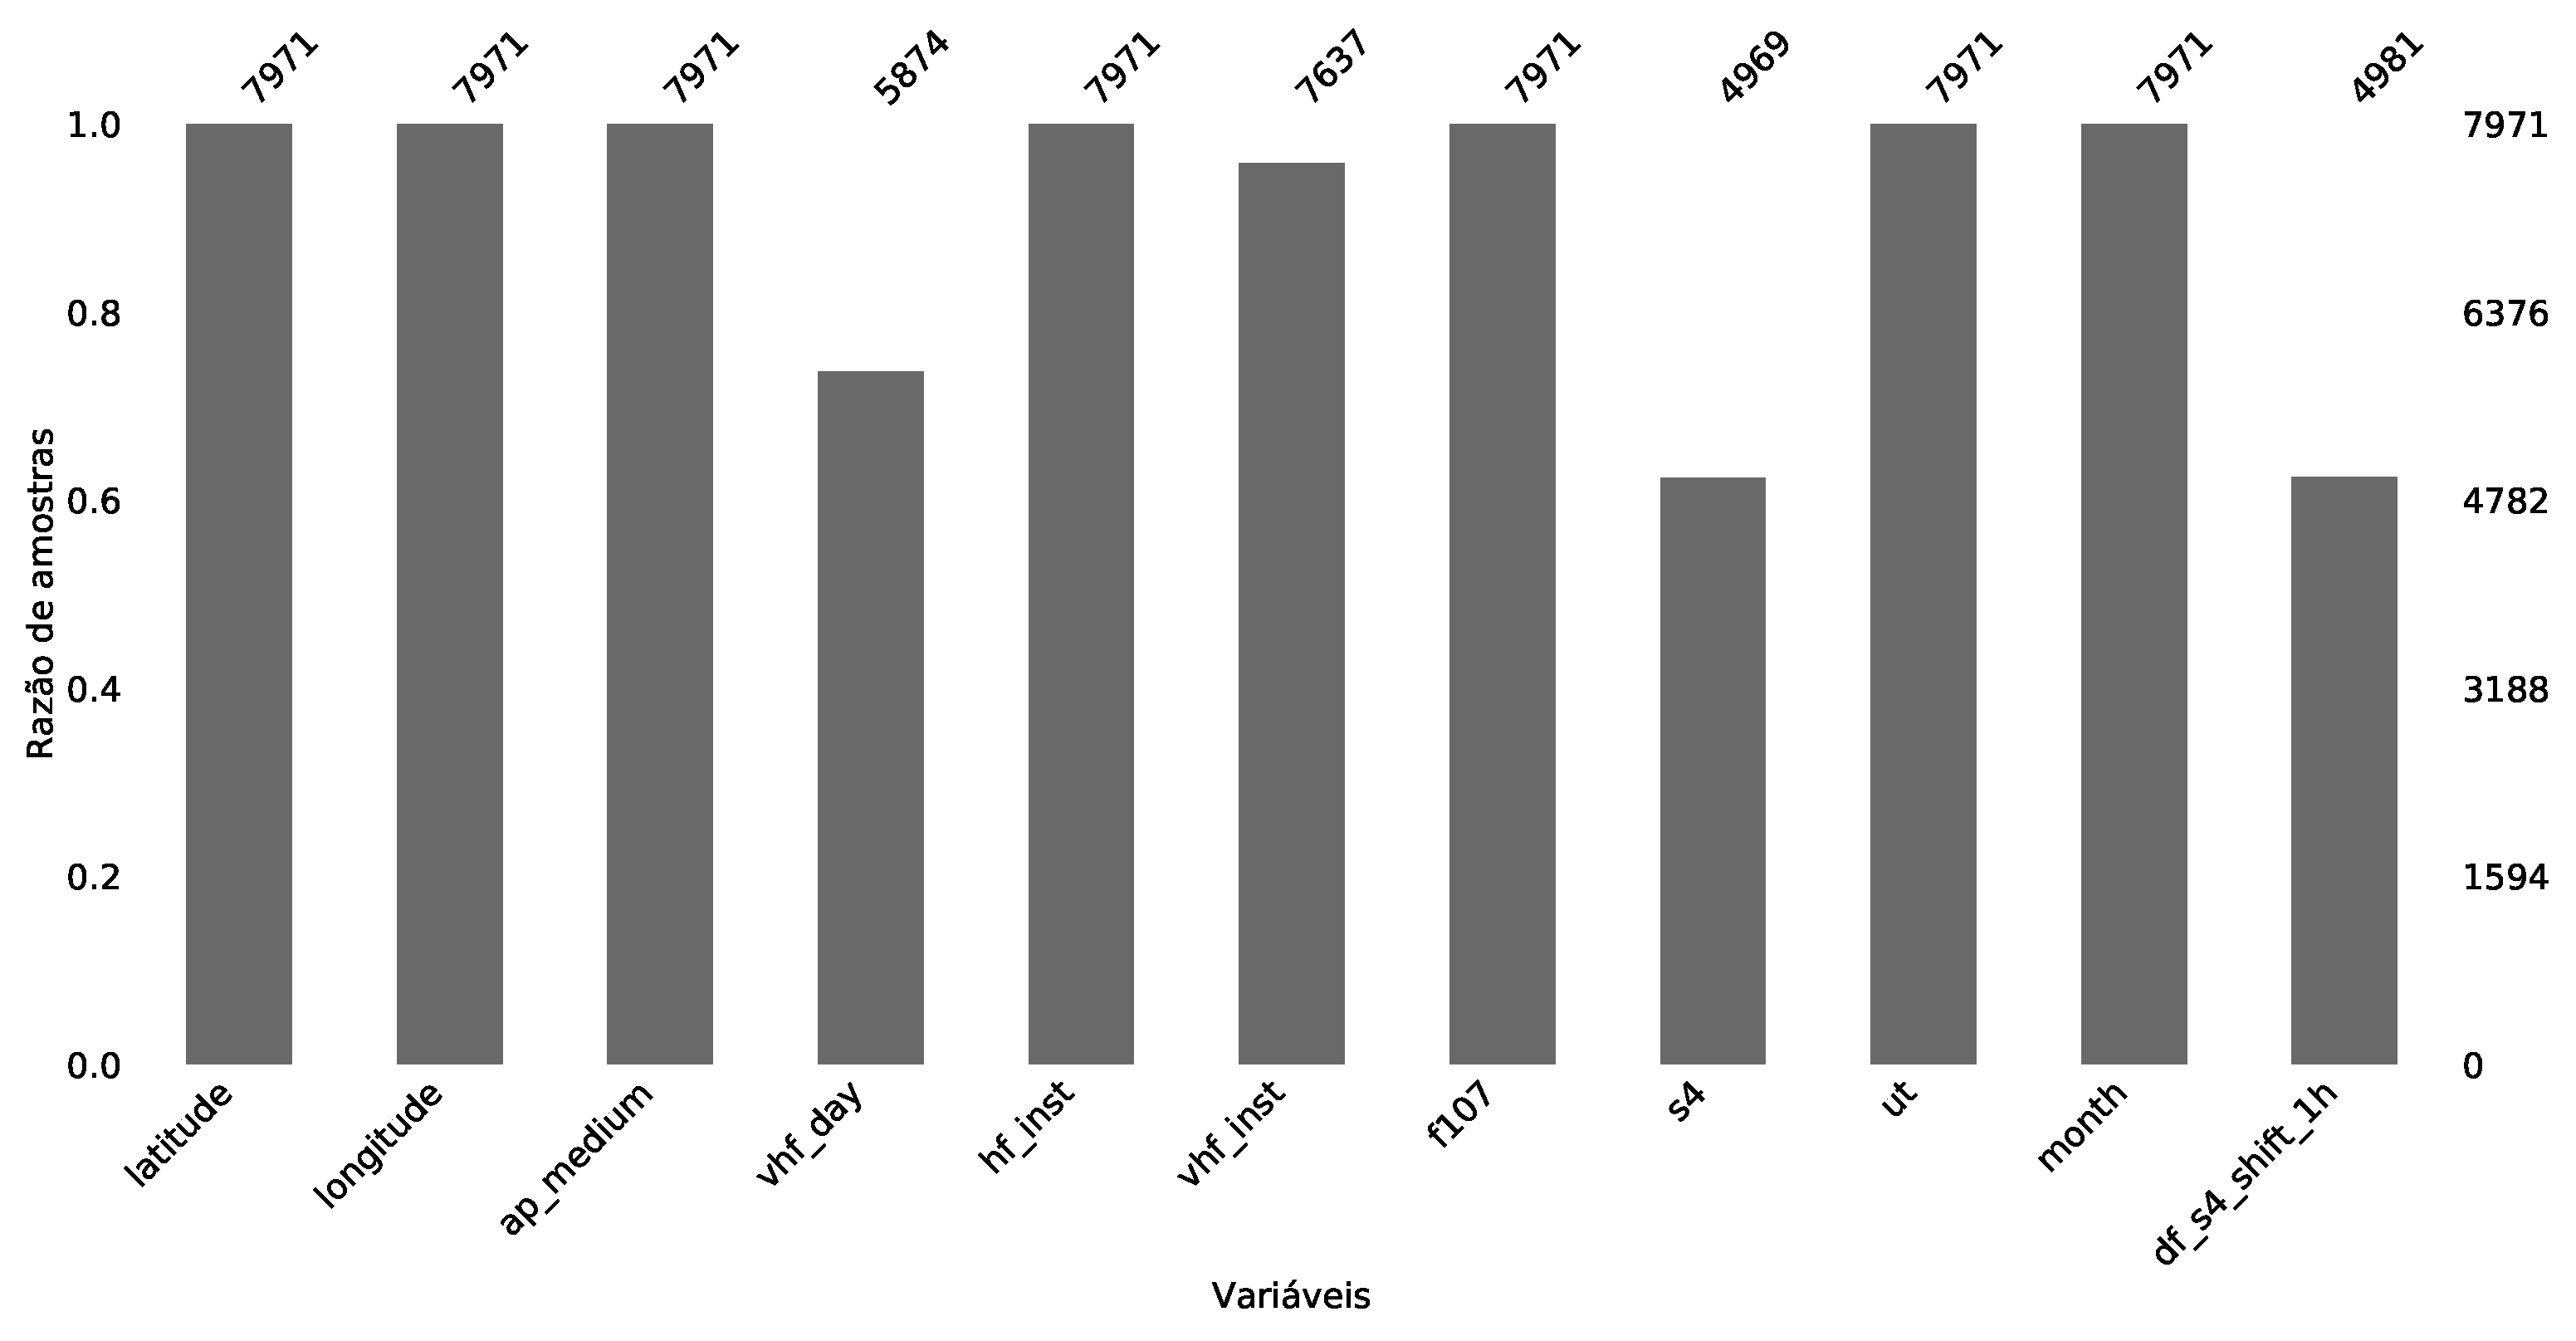
\includegraphics[width=1.2\linewidth]{./Figuras/results-all-stations/nulltotal.eps}}
\caption{Razão e total de dados não nulos por atributo. Fonte: próprio autor.}
\label{fig:nulltotalall}
\end{figure}

Nesta abordagem, somente, foi utilizada validação cruzada com 10 subconjuntos. Esta escolha se deve ao fato do número de amostras não nulas por localização serem variadas. Entretanto, de forma geral, tanto a fase de treinamento quanto a fase de validação são tendenciosas como resultado da não uniformidade do número de amostras por localização. Assim, poder-se-ia descartar os resultados apresentados nesta seção, dados pela Tabelas \ref{tab:results_all_reg} e \ref{tab:results_all_class}  e pelas Figuras \ref{fig:regall} e \ref{fig:classallmik}, porém este é um primeiro resultado interessante para este tipo de abordagem.

\begin{table}[H]
\begin{center}
\begin{tabular}{|c|c|c|}
\hline
Tipo de Validação & mse       & mae   \\ \hline
Validação Cruzada                   & 0,009   & 0,556  \\ \hline
\end{tabular}
\end{center}
\vspace{12pt}
\caption{Resultados para a regressão. Fonte: Próprio autor.}
\label{tab:results_all_reg}
\end{table}

\begin{figure}[H]
\center
\makebox[\textwidth][c]{
\subfigure[fig:regall1][Validação cruzada com 10 subconjuntos.]{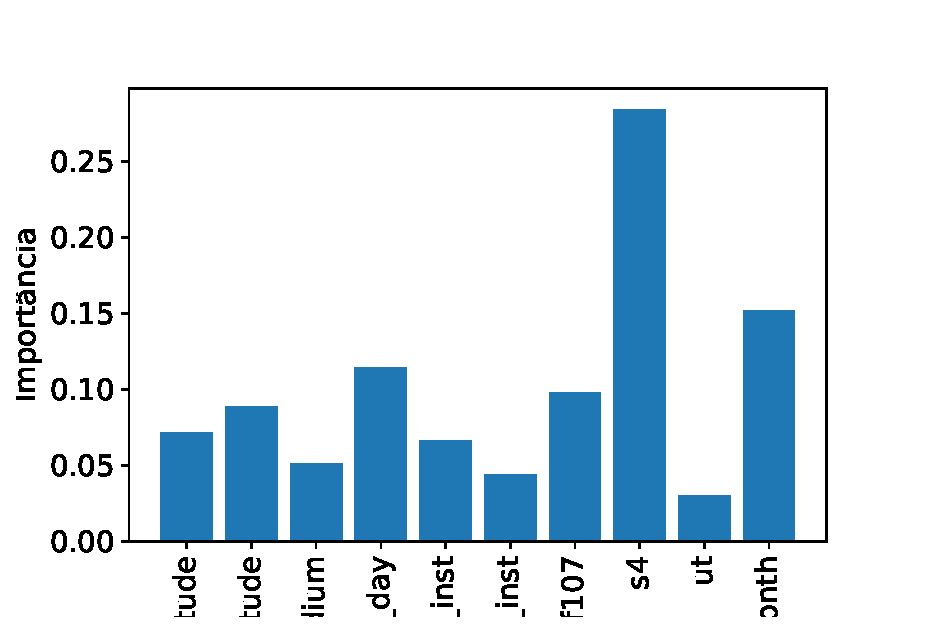
\includegraphics[width=9.5cm]{./Figuras/results-all-stations/regression_kfold_all_2203_4007_importance.eps}}
}
\caption{Importância de cada atributo segundo XGBOOST. Fonte: próprio autor.}\label{fig:regall}
\end{figure}

A Tabela \ref{tab:results_all_class} apresenta a métrica para o resultado obtido com validação cruzada. A Figura\ \ref{fig:classallmik} apresenta a matriz de confusão e um gráfico de barras com a importância das variáveis segundo o XGBOOST.

\begin{table}[H]
\begin{center}
\begin{tabular}{|c|c|}
\hline
Tipo de Validação & precisão balanceada   \\ \hline
Validação Cruzada                   & 0,499   \\ \hline
\end{tabular}
\end{center}
\vspace{12pt}
\caption{Resultados para a classificação. Fonte: Próprio autor.}
\label{tab:results_all_class}
\end{table}

\begin{figure}[H]
\center
\makebox[\textwidth][c]
{
\subfigure[fig:classallmk1][Matriz de Confusão.]{\includegraphics[width=11.5cm]{./Figuras/results-all-stations/classification_kfold_all_2203_4007_confusion_matrix.eps}}
\,\,
\subfigure[fig:classallik2][Importância dos atributos segundo XGBOOST.]{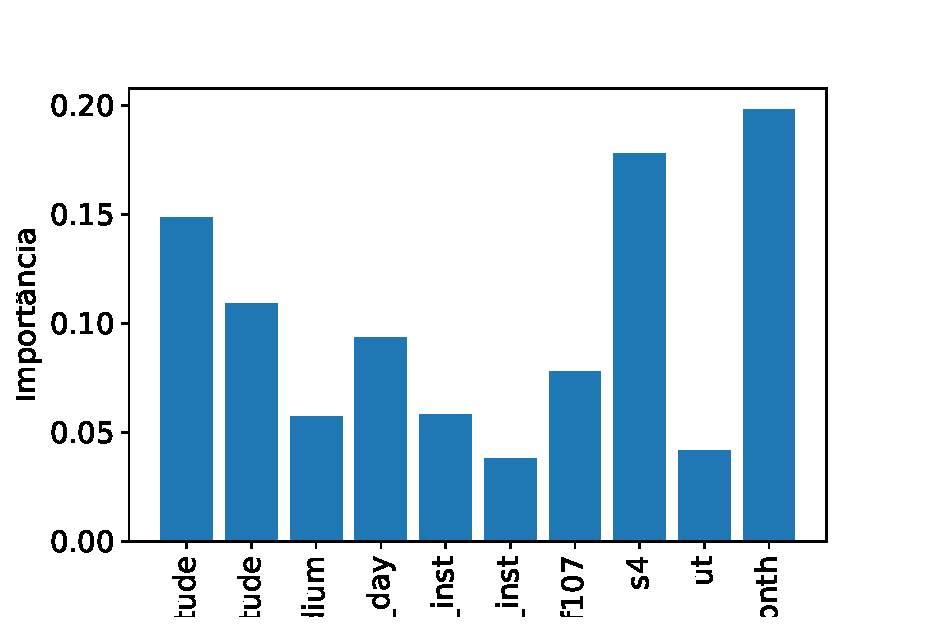
\includegraphics[width=9.5cm]{./Figuras/results-all-stations/classification_kfold_all_2203_4007_importance.eps}}
}
\caption{Resultados para o problema de classificação utilizando de validação cruzada com 10 subconjuntos. Fonte: próprio autor.}
\label{fig:classallmik}
\end{figure}

A busca pela melhoria dos resultados obtidos deve passar por uma etapa natural de expansão horizontal e vertical, isto é, deve-se aumentar o número de atributos preditores, assim como aumentar o número de amostras não nulas. Quanto a questão do número de amostras os objetivos imediatos são a criação de uma base de dados de 2000 à 2018 e a implementação de algoritmo de regressão para expandir o número de amostras de dados de hF. Os objetivos apresentados também se aplicam aos demais modelos explorados nesta proposta.

%Esta última, hF, levanta uma interrogação natural, a disponibilidade de dados aparenta ser melhor em \ref{fig:distributionall} do que em \ref{fig:distribution}. A causa é bem simples, primeiro a base de dados construída apresenta mais dados para o período de 2012 e 2013 em comparação com os demais anos, segundo é feito um processo de descarte de variáveis invalidas para hF em \ref{fig:distributionall} antes da fusão com os dados de $S_4$ o que reduziu drasticamente o número de amostras nulas.
